% Physical Review B manuscript v06, 6 September 2026.
\documentclass[aps,prb,preprint,nofootinbib,longbibliography]{revtex4-2}

\usepackage{amsmath,amssymb}
\usepackage{bm}
\usepackage{graphicx}
\usepackage{hyperref}
\hypersetup{hidelinks}

\newcommand{\Tr}{\operatorname{Tr}}
\newcommand{\Mmod}{\mathfrak{M}}
\newcommand{\ii}{\mathrm{i}}
\newcommand{\E}{\mathbb{E}}
\newcommand{\Wtri}{W_\triangle}
\newcommand{\PhiTri}{\Phi_\triangle}

\newtheorem{theorem}{Theorem}
\newtheorem{proposition}[theorem]{Proposition}
\newtheorem{lemma}[theorem]{Lemma}
\newtheorem{corollary}[theorem]{Corollary}
\newenvironment{proof}{\par\noindent\textit{Proof.}\ }%
{\unskip\nobreak\hfill\(\square\)\par}

\begin{document}

\title{Thermal modular commutators as joint probes of gauge flux and broken
time-reversal symmetry in axial spin networks}

\author{J\'er\^ome Nicolas}
\affiliation{Lyc\'ee Saint-Charles, 5 rue Guy Fabre, 13001 Marseille, France}
\email{jerome.nicolas@ac-aix-marseille.fr}

\date{September 6, 2026}

\begin{abstract}
We establish an exact high-temperature onset law for the thermal modular
commutator on finite, simple, connected, unicyclic spin networks with axial
XXZ--Dzyaloshinskii--Moriya interactions.  The site spins are arbitrary
irreducible representations, and the longitudinal exchanges, longitudinal
fields, and trees grafted onto the cycle are unrestricted.  If the unique
cycle $\gamma$ has length $n$ and contains three distinct marked sites
$A,B,C$ in this cyclic order, then the leading admissible coefficient is
$2(-1)^n h_B\prod_{x\in V(\gamma)}[s_x(s_x+1)/3]
\operatorname{Im}W_\gamma$
at order $\beta^{n+1}$.  The marked sites need not be consecutive.  The proof
uses gauge-flow grading, exact spin moments, and primitive cumulants of the
three marked arcs.  Coefficient extraction also gives an ambient-independent
primitive contribution for each simple cycle that contains $A,B,C$ and an
exact shortest-cycle sum at the first admissible order.  Two independent
mechanisms force all-temperature vanishing within the axial class, namely a
local real structure and physical time-reversal symmetry at zero field.
Axiality is essential.  Transverse on-site fields generate a local,
non-Wilson contribution at order seven on a consecutive three-qubit path,
and an exact seven-cycle example develops this contribution before its
winding term.  We also derive the complete spin-$1/2$ triangle expansion
through sixth order and, in the XY specialization, its first higher Wilson
harmonic.  An exact Jordan--Wigner reconstruction applies to axial XY rings.
For rings with homogeneous hopping magnitudes and a fixed marked-site field,
the computed modular size ratios through $n=70$ approach an exactly known
fermion-parity-string scale.  This last identification is numerical, while
the determinant formula and its temperature asymptotics are analytic.
\end{abstract}

\maketitle

\section{Introduction}
\label{sec:introduction}

Kim \textit{et al.} proposed the modular commutator as a bulk wave-function
probe of chiral central charge \cite{KimEtAl2022PRL} and subsequently
developed its general state-level properties \cite{KimEtAl2022PRB}.  Zou
\textit{et al.} derived its conformal-field-theory dependence on chiral
central charge and the conformal cross ratio \cite{ZouEtAl2022}.  Fan related
entanglement-generated dynamics to the gravitational anomaly
\cite{Fan2022}.  Park, Kim, and Moon proved geometric additivity for the
multipartite configurations they consider in the invertible-state area-law
setting \cite{ParkEtAl2025}.  Gass and Levin introduced
a R\'enyi-like generalization \cite{GassLevin2026}.  Zang studied responses of
entanglement measures under modular flow \cite{Zang2026}.  Zeng found a
robust half-quantized modular commutator at the single-Dirac-node critical
point of the Haldane model and related it to the parity anomaly
\cite{Zeng2026}.  Sheffer
\textit{et al.} used a finite number of replicas with permutation defects to
extract chiral central charge and Hall conductance \cite{ShefferEtAl2026}.
Maity \textit{et al.} applied modular commutators to the Zeeman--Kitaev
honeycomb model and the kagome antiferromagnet with scalar-spin-chirality
perturbations \cite{MaityEtAl2025}.

The same literature delimits the scope.  Gass and Levin constructed lattice
systems with spurious modular commutators, disproving a universal relation to
chiral central charge \cite{GassLevin2024}.  Sun \textit{et al.} showed that
familiar pure-state chirality diagnostics can fail in mixed-state topological
phases \cite{SunEtAl2026}.  These limitations motivate a
narrower question: what can the modular commutator detect exactly in a finite
thermal spin network, without assigning it a quantized or topological
meaning?  Problems 3 and 7 of Ref.~\cite{KimEtAl2022PRB} ask, respectively,
for modular-commutator calculations in further chiral systems, with free
fermions given as one direction, and for a characterization of chirality in
few-body quantum systems.  The present work gives exact finite-temperature
realizations relevant to both questions, first in interacting axial spin
networks and then in axial XY rings through an exact free-fermion
representation.

Within the axial class, we find that a nonzero response requires both a
nonreal Wilson product and broken time-reversal symmetry.  On a unicyclic
network, the leading admissible flux term is a winding process whose order
grows with the cycle length.  In the homogeneous-hopping XY-ring family
studied below, the finite-temperature signal is found numerically to approach
the fermion-parity-string rate over the computed sizes.

This narrower role is naturally connected with recent state-level notions of
chirality and imaginarity.  Vardhan \textit{et al.} define multipartite
chirality by the absence of a product local unitary mapping a state to its
complex conjugate.  They introduce computable nested-commutator witnesses,
including the ordinary tripartite modular commutator, which are not faithful
in general \cite{VardhanEtAl2026}.  Fernandes \textit{et al.} construct
unitary-invariant witnesses of quantum imaginarity for sets of states
\cite{FernandesEtAl2024}.  A distinct many-body notion uses finite-depth
local operations and can remain nontrivial even when tripartite modular
commutators vanish \cite{EllisonEtAl2026}.  Our contribution is not a new
definition of state chirality.  It is an exact thermal resolution, within a
specified interacting spin class, of when the ordinary tripartite modular
commutator must vanish and which gauge-invariant couplings control its first
admissible terms.

We answer this question for axial XXZ--Dzyaloshinskii--Moriya (DM) models.
The antisymmetric exchange interaction was introduced phenomenologically by
Dzyaloshinsky and derived microscopically from spin-orbit-induced
superexchange by Moriya \cite{Dzyaloshinsky1958,Moriya1960}.  For an axial DM
vector, the transverse exchange takes the complex-amplitude form used below.
A phase on one bond depends on the
choice of local spin axes, whereas the product accumulated around a closed
cycle is invariant under independent rotations about the axial direction.
We call this continuous, Abelian obstruction an irreducible spin-orbit gauge
flux, or a Wilson-loop-type phase.  No quantization or topological protection
is implied.

For a faithful state $\rho$ and two regions $X,Y$, we use
\begin{equation}
 \Mmod_\rho(X,Y)
 =\ii\Tr\rho
 \bigl[\widehat{\log\rho_X},\widehat{\log\rho_Y}\bigr].
 \label{eq:def-M}
\end{equation}
Here a hat denotes extension by the identity to $X\cup Y$ after the
complement has been traced out.
This is the modular commutator defined in Eq.~(2) of
Ref.~\cite{KimEtAl2022PRL} and Eq.~(4) of
Ref.~\cite{KimEtAl2022PRB}.  For overlapping $X,Y$, set
$A=X\setminus Y$, $B=X\cap Y$, and $C=Y\setminus X$, after tracing out the
complement of $X\cup Y$.  The two minus signs in the convention
$K_R=-\log\rho_R$ cancel.  Thus Eq.~\eqref{eq:def-M} is not a new
generalization of the state functional.  It is real, antisymmetric under
$X\leftrightarrow Y$, and depends only on $\rho_{X\cup Y}$.

\textit{Principal results.}  First, we turn the local real-structure criterion
of Ref.~\cite{KimEtAl2022PRB} into a graph-theoretic statement for axial spin
networks.  Corollary~\ref{cor:real-gauge} states that if all fundamental Wilson
products are real, then \eqref{eq:def-M} vanishes for every pair of regions and
at every temperature.  Every tree is included.  Independently,
Corollary~\ref{cor:zero-field} shows that physical time reversal forces exact
vanishing whenever all magnetic fields are zero, even in the presence of a
nonreal Wilson product.  A nonzero signal therefore requires a joint
obstruction, namely irreducible gauge flux and broken time-reversal symmetry,
subject
to the chosen tripartition and any remaining spatial symmetries.

Second, Theorem~\ref{thm:unicyclic-onset} gives the leading admissible
coefficient on every finite, simple, connected, unicyclic axial network with
arbitrary irreducible site spins, longitudinal couplings, longitudinal fields,
and grafted trees.  If the unique cycle $\gamma$ has length $n$ and is
oriented through three distinct marked sites $A,B,C$ in this cyclic order,
then
\begin{equation}
 \Mmod_\beta(AB,BC)
 =2(-1)^n\beta^{n+1}h_B
 \left(\prod_{x\in V(\gamma)}\kappa_x\right)
 \operatorname{Im}W_\gamma+O(\beta^{n+2}),
 \qquad
 \kappa_x=\frac{s_x(s_x+1)}3.
 \label{eq:intro-unicyclic}
\end{equation}
The sites need not be consecutive.  Here $AB$ denotes the subsystem
$\{A,B\}$, whether or not it is an edge.  The proof replaces the effective
hopping substitution used in the previous ring argument by a dimensionless
cumulant of the three marked arcs.  Proposition~\ref{prop:primitive-cycle}
then identifies the primitive coefficient carried by any simple cycle in a
general graph, while Corollary~\ref{cor:girth-onset} gives the exact sum over
shortest marked cycles at the first admissible order.  Neither statement is
an all-orders decomposition into independent cycle responses.

Third, Section~\ref{sec:axial-boundary} shows that the axial hypothesis cannot
be removed.  Consecutive transverse on-site fields on a three-qubit path
produce the ambient-independent projected sector
\begin{equation}
 \Pi_{\mathrm{loc}}m_7
 =\frac{J_{AB}^zh_B^z|t_{BC}|^2}{23040}
 \operatorname{Im}(t_{AB}\overline g_Ag_B).
 \label{eq:intro-local-background}
\end{equation}
This is a local open-link gauge invariant, not a Wilson-loop contribution.
The complete $m_7$ is also classified for one explicitly stated
eight-parameter open-path submodel.  An exact seven-cycle example has the
nonzero coefficient $m_7=1/23040$, while its primitive winding term occurs at
order eight.  Two later sections record further controlled directions.  For
a spin-$1/2$ axial triangle, Theorems~\ref{thm:quintic} and
\ref{thm:sextic} determine the complete fifth- and sixth-order coefficients,
and Theorem~\ref{thm:septic} identifies the first higher Wilson harmonic when
$J^z=0$.  For axial XY rings, Proposition~\ref{prop:JW-reconstruction} gives
an exact all-temperature Jordan--Wigner reduction to four Gaussian parity
components and fixed reduced blocks.  The exact parity determinant defines a
scale $r_{\rm P}$.  In the homogeneous-hopping family with a fixed marked-site
field, the computed modular size ratios through $n=70$ approach this scale
over the temperatures studied.  The
determinant identity and its asymptotics are analytic.  The identification of
the modular decay rate remains numerical.

For the oriented triangle $A\to B\to C\to A$, write
$\Wtri=t_{AB}t_{BC}t_{CA}$ and $\PhiTri=\operatorname{Im}\Wtri$.
Fourth, we compare three diagnostics analytically in
the same normalization.
The scalar spin chirality begins at order $\beta^2$ but responds to individual,
gauge-removable DM amplitudes.  A product of oriented two-point coherences
begins at order $\beta^3$ and measures $\PhiTri$ without a field.  The modular
commutator begins at order $\beta^4$ and measures $h_B\PhiTri$.  As a direct
flux meter, the coherence loop therefore has a lower-order onset and requires
only three two-point coherences.
The distinct point of \eqref{eq:def-M} is that it is a functional of the state
and the tripartition alone.  No bond operators, spin axes, or cycle need be
specified in its definition.

The paper is organized as follows.  Section~\ref{sec:state-functional}
reviews the state-level structure and derives the two exact vanishing
mechanisms for axial networks.  Section~\ref{sec:unicyclic} proves the
arbitrary-spin unicyclic theorem.  Section~\ref{sec:primitive-cycles}
isolates primitive cycle sectors on general graphs, and
Sec.~\ref{sec:axial-boundary} establishes the necessity of axiality.
Section~\ref{sec:triangle-refinements} gives the qubit triangle refinements.
Section~\ref{sec:free-fermion-rings} develops the exact Jordan--Wigner
reconstruction and the numerical attenuation study.  The final sections
compare three chirality diagnostics, discuss finite-temperature behavior and
measurement, and state the limits of the results.

\section{State structure and exact vanishing in axial networks}
\label{sec:state-functional}

Let
\(
\mathcal H=\bigotimes_{x\in V}\mathcal H_x
\)
be finite dimensional, and let $\rho>0$ be a faithful state.  For a region
$X\subseteq V$, write $\rho_X=\Tr_{X^c}\rho$.  If $O_X$ acts on
$\mathcal H_X$, its extension by the identity to $\mathcal H$ is denoted by
$\widehat O_X$.

\subsection{Local-unitary and antiunitary transformations}

The transformation laws below use the site-by-site specialization of the
region-by-region product unitaries surrounding Eqs.~(8) and (9) of
Ref.~\cite{KimEtAl2022PRB}.  No invariance under a circuit crossing the
region boundaries is used.

\begin{lemma}[Transformation laws]
\label{lem:symmetries}
Let $X,Y\subseteq V$.

If $U=\bigotimes_xU_x$ is a product of local unitaries, then
\begin{equation}
 \Mmod_{U\rho U^\dagger}(X,Y)=\Mmod_\rho(X,Y).
 \label{eq:local-unitary-invariance}
\end{equation}
If $\mathcal A=VK$ is an antiunitary compatible with the product structure,
where $V$ is a product of local unitaries and $K$ is complex conjugation in a
product basis, then
\begin{equation}
 \Mmod_{\mathcal A\rho\mathcal A^{-1}}(X,Y)
 =-\Mmod_\rho(X,Y).
 \label{eq:antiunitary-oddness}
\end{equation}
\end{lemma}

\begin{proof}
The reduced state of $U\rho U^\dagger$ on $X$ is
$U_X\rho_XU_X^\dagger$.  Spectral functional calculus therefore gives
\(
\log(U_X\rho_XU_X^\dagger)=U_X(\log\rho_X)U_X^\dagger
\),
and Eq.~\eqref{eq:local-unitary-invariance} follows from cyclicity of the
trace.

It is enough to prove Eq.~\eqref{eq:antiunitary-oddness} for $K$.  Put
$Z=\Tr\rho[\widehat{\log\rho_X},\widehat{\log\rho_Y}]$.  Since the
commutator is anti-Hermitian, $Z$ is purely imaginary.  Complex conjugation
commutes with partial traces and spectral functional calculus, whence
\begin{equation*}
 \Mmod_{\overline\rho}(X,Y)
 =\ii\,\overline{Z}=-\ii Z=-\Mmod_\rho(X,Y).
\end{equation*}
The local-unitary part $V$ is handled by
Eq.~\eqref{eq:local-unitary-invariance}.
\end{proof}

\subsection{Vanishing from a local real structure}

The following criterion is likewise a known state-level property of the
modular commutator \cite{KimEtAl2022PRB}.  Its proof is included to make clear
which part of the later graph-theoretic corollary is model independent.

\begin{proposition}[Local real-structure criterion]
\label{prop:real-structure}
Suppose that local unitaries $U_x$ and a product basis exist such that
$U\rho U^\dagger$ is real in that basis, where $U=\bigotimes_xU_x$.  Then
\begin{equation}
 \Mmod_\rho(X,Y)=0
 \label{eq:real-structure-vanishing}
\end{equation}
for every pair of regions $X,Y\subseteq V$.
\end{proposition}

\begin{proof}
By Lemma~\ref{lem:symmetries}, it is enough to consider a real state $\rho$.
Because $\rho$ is Hermitian, its matrix is then real symmetric.  Partial
traces in the chosen product basis preserve reality and symmetry, and so does
spectral functional calculus.  Consequently,
$\widehat{\log\rho_X}$ and $\widehat{\log\rho_Y}$ are real symmetric,
whereas their commutator is real antisymmetric.  If $S$ is symmetric and $A$
is antisymmetric, then
\(
\Tr(SA)=\Tr[(SA)^T]=-\Tr(AS)=-\Tr(SA)
\).
Taking $S=\rho$ proves Eq.~\eqref{eq:real-structure-vanishing}.
\end{proof}

Reference~\cite{KimEtAl2022PRB} also noted the resulting vanishing for
reduced Gibbs states of stoquastic Hamiltonians.  Corollary
\ref{cor:real-gauge} below has a different, model-specific purpose: it gives
a necessary and sufficient cycle criterion for when an axial XXZ--DM
Hamiltonian can be made real by local $U(1)$ rotations, even though its bond
amplitudes are complex in the original $S^z$ basis.

\subsection{Axial XXZ--DM networks and Wilson products}
\label{sec:axial}

At each vertex $x$, let $\mathcal H_x$ carry the irreducible spin-$s_x$
representation, where
\begin{equation}
 s_x\in\left\{\frac12,1,\frac32,\ldots\right\},
 \qquad
 \kappa_x=\frac{s_x(s_x+1)}3.
 \label{eq:kappa-definition}
\end{equation}
Consider the axial Hamiltonian
\begin{equation}
 H=\sum_{\{x,y\}\in E}
 \left[
 \frac12\left(
 t_{xy}S_x^+S_y^-+\overline{t_{xy}}S_x^-S_y^+
 \right)
 +J_{xy}^zS_x^zS_y^z
 \right]
 -\sum_{x\in V}h_xS_x^z.
 \label{eq:axial-H}
\end{equation}
Here $t_{xy}\in\mathbb C$, $J_{xy}^z=J_{yx}^z\in\mathbb R$, and
$h_x\in\mathbb R$.  An orientation is chosen for each edge, with
\begin{equation}
 t_{yx}=\overline{t_{xy}},
 \qquad
 t_{xy}=J_{xy}^{\perp}+\ii D_{xy}^z.
 \label{eq:t-definition}
\end{equation}
For the local rotation
\begin{equation}
 U_{\bm\varphi}
 =\exp\left(\ii\sum_x\varphi_xS_x^z\right),
 \label{eq:gauge-unitary}
\end{equation}
one has
\begin{equation}
 U_{\bm\varphi}H(t,J^z,h)U_{\bm\varphi}^\dagger
 =H(t^{\bm\varphi},J^z,h),
 \qquad
 t_{xy}^{\bm\varphi}
 =t_{xy}e^{\ii(\varphi_x-\varphi_y)}.
 \label{eq:gauge-action}
\end{equation}

For an oriented cycle
\(
\gamma=(x_1,x_2,\ldots,x_n,x_1)
\), define
\begin{equation}
 W_\gamma
 =\prod_{j=1}^nt_{x_jx_{j+1}},
 \qquad
 \vartheta_\gamma=\arg W_\gamma,
 \qquad
 \Phi_\gamma=\operatorname{Im}W_\gamma.
 \label{eq:Wilson-definitions}
\end{equation}
The product $W_\gamma$ and, when nonzero, its phase are invariant under
Eq.~\eqref{eq:gauge-action}.

\begin{corollary}[Axial real-gauge criterion]
\label{cor:real-gauge}
Remove all edges for which $t_{xy}=0$.  A gauge of the form
Eq.~\eqref{eq:gauge-unitary} that makes every remaining $t_{xy}$ real exists
if and only if
\begin{equation}
 W_\gamma\in\mathbb R
 \label{eq:real-Wilson-products}
\end{equation}
for every fundamental cycle associated with a spanning forest, equivalently
for every simple oriented cycle of the remaining graph.  If this condition holds,
then the Gibbs state $\rho_\beta=e^{-\beta H}/\Tr e^{-\beta H}$ satisfies
\begin{equation}
 \Mmod_\beta(X,Y)=0
 \label{eq:axial-all-temperature-vanishing}
\end{equation}
for all $X,Y$ and all finite $\beta$.  In particular,
Eq.~\eqref{eq:axial-all-temperature-vanishing} holds on every tree.
\end{corollary}

\begin{proof}
If every transformed coupling is real, every cycle product is real.  For the
converse, choose a spanning forest.  On each component, fix the phase at one
root and determine the remaining vertex phases recursively so that the
couplings on the forest are real.  Each edge outside the forest closes a
unique fundamental cycle.  Its transformed phase is the phase accumulated
around that cycle, which belongs to $\pi\mathbb Z$ by
Eq.~\eqref{eq:real-Wilson-products}.  Hence every remaining coupling is real.

In this gauge the matrix of $H$ is real in the product $S^z$ basis, as are
$e^{-\beta H}$ and the normalized Gibbs state.  Proposition
\ref{prop:real-structure} completes the proof.
\end{proof}

Complex conjugation $K$ in the product $S^z$ basis and physical time reversal
$\Theta$ are distinct antiunitary operations.  Their parameter actions are
\begin{align}
 K H(t,J^z,h)K^{-1}&=H(\overline t,J^z,h),
 \label{eq:K-action}\\
 \Theta H(t,J^z,h)\Theta^{-1}&=H(t,J^z,-h).
 \label{eq:Theta-action}
\end{align}
The DM interaction is bilinear in spin operators and is therefore even under
physical time reversal.  Lemma~\ref{lem:symmetries} gives
\begin{align}
 \Mmod_\beta(\overline t,J^z,h)
 &=-\Mmod_\beta(t,J^z,h),
 \label{eq:M-K-odd}\\
 \Mmod_\beta(t,J^z,-h)
 &=-\Mmod_\beta(t,J^z,h).
 \label{eq:M-Theta-odd}
\end{align}

Equation~\eqref{eq:M-Theta-odd} gives a second exact vanishing mechanism that
does not follow from the real-gauge criterion.

\begin{corollary}[Zero-field vanishing]
\label{cor:zero-field}
For the axial Hamiltonian \eqref{eq:axial-H}, if $h_x=0$ at every vertex,
then
\begin{equation}
 \Mmod_\beta(X,Y)=0
 \label{eq:zero-field-vanishing}
\end{equation}
for all regions $X,Y$ and all finite $\beta$, irrespective of the Wilson
products.
\end{corollary}

\begin{proof}
At zero field the Gibbs state is invariant under physical time reversal.
Antiunitary oddness then identifies $\Mmod_\beta$ with its negative.
\end{proof}

Corollaries~\ref{cor:real-gauge} and \ref{cor:zero-field} are independent.  A
nonreal Wilson product obstructs the axial real gauge but does not by itself
produce a modular signal.  Conversely, a magnetic field breaks physical time
reversal but produces no signal on a tree.  Even when both obstructions are
present, the particular regions or a reflection symmetry may still force an
additional cancellation.

\section{Arbitrary-spin onset on finite unicyclic networks}
\label{sec:unicyclic}

We now determine the first coefficient allowed by gauge invariance and physical
time reversal on a finite unicyclic graph.  The result applies to arbitrary
irreducible site spins.  It also allows arbitrary longitudinal exchanges,
longitudinal fields, and trees grafted onto the unique cycle.  All Hamiltonian
parameters are held fixed as $\beta\to0$.

Let $G=(V,E)$ be finite, simple, connected, and unicyclic.  Denote its unique
cycle by $\gamma$ and its length by $n\geq3$.  Choose three distinct vertices
$A,B,C\in V(\gamma)$.  Orient $\gamma$ so that they occur in the cyclic order

\begin{equation}
 \gamma=(A,\ldots,B,\ldots,C,\ldots,A).
 \label{eq:marked-cycle-order}
\end{equation}

For this orientation, set

\begin{equation}
 W_\gamma=\prod_{(x,y)\in\gamma}t_{xy}.
 \label{eq:unicyclic-W}
\end{equation}

The notation $AB$ below means the subsystem $\{A,B\}$.  It does not assert
that $A$ and $B$ are adjacent.  The same convention applies to $BC$.

\begin{theorem}[Arbitrary-spin unicyclic onset]
\label{thm:unicyclic-onset}
For the axial Hamiltonian \eqref{eq:axial-H}, let every $\mathcal H_x$ carry
the irreducible spin-$s_x$ representation, with $\kappa_x$ defined in
Eq.~\eqref{eq:kappa-definition}.  Assume $t_{xy}\in\mathbb C$ with
$t_{yx}=\overline{t_{xy}}$, $J^z_{xy}\in\mathbb R$, and $h_x\in\mathbb R$.
Then every Taylor coefficient of
$\Mmod_\beta(AB,BC)$ through order $n$ vanishes, and

\begin{equation}
 \boxed{
 \Mmod_\beta(AB,BC)
 =2(-1)^n\beta^{n+1}h_B
 \left(\prod_{x\in V(\gamma)}\kappa_x\right)
 \operatorname{Im}W_\gamma
 +O(\beta^{n+2}) .}
 \label{eq:unicyclic-onset}
\end{equation}

No coupling is assumed to be nonzero.  Equation~\eqref{eq:unicyclic-onset}
is therefore a statement about the leading admissible coefficient.  Its
displayed coefficient can vanish for a particular Hamiltonian.
\end{theorem}

The proof occupies the rest of this section.  We first isolate the only
possible monomial at order $n+1$.  We then evaluate its coefficient by
reducing the cycle to three primitive arc cumulants.  This second step is
needed because tracing out an arc generates multispin operators in addition
to its endpoint hopping.

\subsection{Gauge-flow grading and pruning}

Write the analytic expansion near the maximally mixed state as

\begin{equation}
 \Mmod_\beta(AB,BC)=\sum_{q\geq0}\beta^q m_q.
 \label{eq:unicyclic-series}
\end{equation}

Finite dimensionality makes this series convergent in a neighborhood of
$\beta=0$.  The identity $\rho_\beta(H)=\rho_1(\beta H)$ shows that $m_q$ is
homogeneous of total degree $q$ in the Hamiltonian parameters.

For coefficient extraction, first write $t_e=x_e+\ii y_e$.  Each $m_q$ is a
real polynomial in $x,y,J^z,h$.  Complexify this polynomial and make the
invertible change of variables

\begin{equation}
 z_e=x_e+\ii y_e,
 \qquad
 w_e=x_e-\ii y_e.
 \label{eq:formal-complexification}
\end{equation}

The variables $z_e$ and $w_e$ are now algebraically independent.  The
physical coefficient is recovered on $w_e=\overline{z_e}$.  Gauge invariance
under the vertex torus is a polynomial identity, so distinct torus characters
vanish coefficientwise.  Equations~\eqref{eq:M-K-odd} and
\eqref{eq:M-Theta-odd} give the polynomial identities

\begin{align}
 m_q(w,z,J^z,h)&=-m_q(z,w,J^z,h),
 \label{eq:formal-K-oddness}\\
 m_q(z,w,J^z,-h)&=-m_q(z,w,J^z,h).
 \label{eq:formal-Theta-oddness}
\end{align}

This formalization also makes every edge multidegree unambiguous.

Fix an orientation of each edge.  For a monomial, let $a_e$ and $b_e$ be the
exponents of $z_e$ and $w_e$, and define the integral edge flow

\begin{equation}
 d_e=a_e-b_e.
 \label{eq:edge-flow}
\end{equation}

Local rotations about the $z$ axis leave the modular commutator invariant.
Character independence under this torus action means that the coefficient of
a monomial can be nonzero only if

\begin{equation}
 \operatorname{div}d=0
 \label{eq:flow-divergence}
\end{equation}

at every vertex.  On a unicyclic graph, any integral flow satisfying
Eq.~\eqref{eq:flow-divergence} vanishes on every bridge.  Its restriction to
$\gamma$ is $k$ times the consistently oriented unit flow for some
$k\in\mathbb Z$.  This follows by removing the cycle edges, starting at a
leaf of each remaining tree, and imposing zero divergence inward.  Zero
divergence on the cycle then makes all oriented cycle values equal.

Let $D_{\mathrm{hop}}=\sum_e(a_e+b_e)$ be the hopping degree.
Equation~\eqref{eq:formal-K-oddness} removes the sector $d=0$.  Indeed, every
monomial in that sector is fixed by $z\leftrightarrow w$ after identical
factors are collected.  Every surviving monomial thus has $k\neq0$, and

\begin{equation}
 D_{\mathrm{hop}}
 \geq\sum_e|d_e|
 =n|k|
 \geq n.
 \label{eq:hopping-lower-bound}
\end{equation}

Equation~\eqref{eq:formal-Theta-oddness} says that the total field degree of
every surviving monomial is odd and in particular is at least one.  In the
physical Hamiltonian, this identity follows because time reversal leaves $t$
and $J^z$ fixed in the parameterization used here, sends $h$ to $-h$, and
reverses the modular commutator.  Equations~\eqref{eq:unicyclic-series} and
\eqref{eq:hopping-lower-bound} now imply

\begin{equation}
 m_q=0\qquad(0\leq q\leq n).
 \label{eq:unicyclic-low-orders-zero}
\end{equation}

Equality in the degree bound at order $n+1$ is rigid.  The flow is one unit
around $\gamma$, one oriented hopping monomial occurs on every cycle edge,
and exactly one longitudinal field occurs.  There is no degree
left for a longitudinal exchange, a bridge hopping, or a neutral return.
After combining the two conjugate orientations, one obtains

\begin{equation}
 m_{n+1}=\operatorname{Im}W_\gamma\sum_{x\in V}c_xh_x
 \label{eq:unicyclic-leading-classification}
\end{equation}

with real constants $c_x$ that can a priori depend on the graph and its site
spins.

Equation~\eqref{eq:unicyclic-leading-classification} also proves a useful
pruning statement.  Extract the coefficient of $h_xW_\gamma$ and set every
parameter absent from that monomial to zero.  Every grafted tree then becomes
a decoupled tensor factor.  If $x\notin V(\gamma)$, the remaining field acts
on a factor disjoint from $ABC$, so the reduced state on $ABC$ is independent
of $h_x$ and $c_x=0$.  If $x\in V(\gamma)$, every off-cycle normalized trace
equals one.  The coefficient is therefore exactly the coefficient of the
isolated marked cycle, and the remaining constants depend only on the cycle
spins.  We may work with $H_\gamma$ from now on.

\subsection{Three-site expansion through fourth order}
\label{sec:three-site-expansion}

The triangular seed below uses a general local expansion that we record here.
In this subsection, $H$ is a Hamiltonian on
$\mathcal H_A\otimes\mathcal H_B\otimes\mathcal H_C$.  A scalar can be
subtracted from $H$ without changing its Gibbs state, so we take
$\tau(H)=0$, where

\begin{equation}
 \tau(O)=\frac1d\operatorname{Tr}O,
 \qquad
 d=\dim(\mathcal H_A\otimes\mathcal H_B\otimes\mathcal H_C).
 \label{eq:normalized-trace}
\end{equation}

For $X\subseteq ABC$, let $X^c$ denote the complement inside $ABC$ and
introduce the trace-preserving conditional expectation

\begin{equation}
 \E_X(O)
 =\frac{1}{d_{X^c}}\operatorname{Tr}_{X^c}(O)\otimes I_{X^c}.
 \label{eq:conditional-expectation}
\end{equation}

Set

\begin{equation}
 r_\beta=d\rho_\beta
 =\frac{e^{-\beta H}}{\tau(e^{-\beta H})},
 \qquad
 L_X(\beta)=\log\E_X(r_\beta).
 \label{eq:r-and-L}
\end{equation}

Since
$\E_X(r_\beta)=d_X\rho_{\beta,X}\otimes I_{X^c}$,
$L_X$ differs from the extended operator
$\widehat{\log\rho_{\beta,X}}$ only by a scalar.  Hence

\begin{equation}
 \Mmod_\beta(AB,BC)
 =\ii\tau\left(r_\beta
 [L_{AB}(\beta),L_{BC}(\beta)]\right).
 \label{eq:M-normalized}
\end{equation}

The normalized Gibbs density has the expansion

\begin{equation}
 r_\beta
 =I-\beta H
 +\frac{\beta^2}{2}
 \left(H^2-\tau(H^2)I\right)
 +O(\beta^3).
 \label{eq:r-expansion}
\end{equation}

Define

\begin{equation}
 P=\E_{AB}(H),
 \qquad
 Q=\E_{BC}(H),
 \label{eq:PQ}
\end{equation}

and, modulo scalar multiples of the identity,

\begin{align}
 A_2&=\frac12\left(\E_{AB}(H^2)-P^2\right),
 \label{eq:A2}\\
 B_2&=\frac12\left(\E_{BC}(H^2)-Q^2\right).
 \label{eq:B2}
\end{align}

Expanding the logarithms gives

\begin{align}
 L_{AB}(\beta)&=-\beta P+\beta^2A_2+O(\beta^3),
 \label{eq:LAB-expansion}\\
 L_{BC}(\beta)&=-\beta Q+\beta^2B_2+O(\beta^3).
 \label{eq:LBC-expansion}
\end{align}

\begin{lemma}[Expansion through fourth order]
\label{lem:fourth-order-expansion}
The coefficient of $\beta^2$ in the modular commutator vanishes.  The next
two coefficients are

\begin{align}
 [\beta^3]\Mmod_\beta(AB,BC)
 &=-\ii\tau\bigl(H[P,Q]\bigr),
 \label{eq:m3-general}\\
 [\beta^4]\Mmod_\beta(AB,BC)
 &=\ii\tau\left[
 \frac12H^2[P,Q]
 +H\bigl([P,B_2]+[A_2,Q]\bigr)
 \right].
 \label{eq:m4-general}
\end{align}
\end{lemma}

\begin{proof}
Insert Eqs.~\eqref{eq:r-expansion} through
\eqref{eq:LBC-expansion} into Eq.~\eqref{eq:M-normalized}.  At order
$\beta^2$ one obtains $\ii\tau([P,Q])=0$.  At order $\beta^3$, every bare
commutator has zero trace, leaving Eq.~\eqref{eq:m3-general}.  At order
$\beta^4$, terms involving the third-order coefficients of $L_{AB}$ or
$L_{BC}$ again occur as bare commutators.  The remaining contributions are
those in Eq.~\eqref{eq:m4-general}.
\end{proof}

\subsection{Local spin moments and the triangular seed}
\label{sec:arbitrary-spin-triangle}

Let

\begin{equation}
 \tau_x(O)=\frac{1}{2s_x+1}\operatorname{Tr}_x O.
 \label{eq:local-normalized-trace}
\end{equation}

Rotational invariance of the normalized trace and the spin commutation
relations give

\begin{align}
 \tau_x(S_x^a)&=0,
 \label{eq:spin-first-moment}\\
 \tau_x(S_x^aS_x^b)&=\kappa_x\delta_{ab},
 \label{eq:spin-second-moment}\\
 \tau_x(S_x^aS_x^bS_x^c)
 &=\frac{\ii\kappa_x}{2}\varepsilon_{abc}.
 \label{eq:spin-third-moment}
\end{align}

For completeness, the second moment is an invariant rank-two tensor.  Its
trace over $a=b$ is $s_x(s_x+1)$, which gives
Eq.~\eqref{eq:spin-second-moment}.  The invariant rank-three tensor is
antisymmetric.  Taking the trace of
$[S_x^a,S_x^b]S_x^c=\ii\varepsilon_{abd}S_x^dS_x^c$ fixes its coefficient
and proves Eq.~\eqref{eq:spin-third-moment}.  In the ladder basis these
identities read

\begin{equation}
 \tau_x(S_x^+S_x^-)=\tau_x(S_x^-S_x^+)=2\kappa_x,
 \label{eq:spin-ladder-second-moment}
\end{equation}

while the six orderings of $S_x^+,S_x^-,S_x^z$ have normalized trace
$+\kappa_x$ or $-\kappa_x$, three of each.

\begin{proposition}[Arbitrary-spin triangular seed]
\label{prop:arbitrary-spin-triangle}
For the isolated three-site axial triangle oriented as
$A\to B\to C\to A$, with arbitrary irreducible spins and arbitrary axial
couplings,

\begin{equation}
 \Mmod_\beta(AB,BC)
 =-2\beta^4h_B\kappa_A\kappa_B\kappa_C
 \operatorname{Im}(t_{AB}t_{BC}t_{CA})+O(\beta^5).
 \label{eq:arbitrary-spin-triangle}
\end{equation}

The coefficient is independent of $h_A$, $h_C$, and all $J^z$ couplings.
\end{proposition}

\begin{proof}
Homogeneity, gauge invariance, conjugation oddness, and field oddness give

\begin{equation}
 [\beta^4]\Mmod_\beta(AB,BC)
 =(c_Ah_A+c_Bh_B+c_Ch_C)
 \operatorname{Im}(t_{AB}t_{BC}t_{CA}).
 \label{eq:triangle-arbitrary-classification}
\end{equation}

There is no degree available for $J^z$.  Evaluate the three constants at the
unit-amplitude parameter point

\begin{equation}
 t_{AB}=t_{BC}=1,
 \qquad
 t_{CA}=\ii,
 \qquad
 J^z=0.
 \label{eq:arbitrary-triangle-point}
\end{equation}

Use $P,Q,A_2,B_2$ from Eqs.~\eqref{eq:PQ} through \eqref{eq:B2} and write

\begin{align}
 T_0&=\frac{\ii}{2}\tau\bigl(H^2[P,Q]\bigr),
 \label{eq:triangle-T0}\\
 T_1&=\ii\tau\bigl(H[P,B_2]\bigr),
 \label{eq:triangle-T1}\\
 T_2&=\ii\tau\bigl(H[A_2,Q]\bigr).
 \label{eq:triangle-T2}
\end{align}

Lemma~\ref{lem:fourth-order-expansion} gives
$[\beta^4]\Mmod_\beta=T_0+T_1+T_2$.  Differentiation with respect to one
field at zero field gives the exact contraction table

\begin{equation}
\begin{array}{c|ccc|c}
 r&\partial_{h_r}T_0&\partial_{h_r}T_1&\partial_{h_r}T_2
 &\partial_{h_r}m_4\\
 \hline
 A&0&0&0&0\\
 B&2K_\triangle&-2K_\triangle&-2K_\triangle&-2K_\triangle\\
 C&0&0&0&0
\end{array}
\qquad
K_\triangle=\kappa_A\kappa_B\kappa_C.
 \label{eq:arbitrary-spin-contraction-table}
\end{equation}

We justify the lift from the explicit spin-$1/2$ contraction in
Appendix~\ref{app:pauli-certificate}.  In every nonzero square-free
contraction of $h_r t_{AB}t_{BC}t_{CA}$, each vertex distinct from $r$
carries one $S^+$ and one $S^-$.  The vertex $r$ carries one each of
$S^+$, $S^-$, and $S^z$.  If a conditional expectation splits the letters
at a vertex among two normalized traces, one factor contains a single
traceless generator and the contraction vanishes.  Every surviving
contraction therefore uses exactly one of
Eqs.~\eqref{eq:spin-ladder-second-moment} and
\eqref{eq:spin-third-moment} at each vertex.  Its ratio to the spin-$1/2$
value is $4\kappa_x$ at vertex $x$.  Multiplying every entry of the qubit
table by
$\prod_{x\in\{A,B,C\}}4\kappa_x$ gives
Eq.~\eqref{eq:arbitrary-spin-contraction-table}.  Summing its three columns
proves Eq.~\eqref{eq:arbitrary-spin-triangle}.
\end{proof}

This argument lifts the square-free contraction, not the Pauli
anticommutator identities.  Only the second and third normalized spin
moments are used.

\subsection{Primitive cumulants of the three marked arcs}

Split the oriented cycle into the three internally disjoint arcs

\begin{equation}
 P_1:A\longrightarrow B,
 \qquad
 P_2:B\longrightarrow C,
 \qquad
 P_3:C\longrightarrow A.
 \label{eq:three-marked-arcs}
\end{equation}

Let their lengths be $\ell_1,\ell_2,\ell_3\geq1$, so that
$\ell_1+\ell_2+\ell_3=n$.  Put $U=\{A,B,C\}$ and
$I=V(\gamma)\setminus U$.  With

\begin{equation}
 \tau_I(O)=\frac{1}{d_I}\operatorname{Tr}_I O,
 \qquad
 d_I=\prod_{x\in I}(2s_x+1),
 \label{eq:internal-normalized-trace}
\end{equation}

the normalized partial trace over $I$ defines

\begin{align}
 G(\beta)&=\tau_I(e^{-\beta H_\gamma}),
 \label{eq:arc-G}\\
 Q(\beta)&=-\log G(\beta).
 \label{eq:arc-Q}
\end{align}

The physical reduced state on $U$ is
$G/\operatorname{Tr}_UG$.  Define the real-analytic functional near $Q=0$

\begin{equation}
 \mathcal F(Q)
 =\Mmod_{e^{-Q}/\operatorname{Tr}_Ue^{-Q}}(AB,BC).
 \label{eq:triangle-functional}
\end{equation}

Then $\Mmod_\beta(AB,BC)=\mathcal F(Q(\beta))$.  The dimensionless
definition \eqref{eq:arc-Q} is essential.  The composed functional is
$\mathcal F(Q)$, not the same functional evaluated on
$-\beta^{-1}\log G$.

Consider an oriented arc

\begin{equation}
 P=(v_0=u,v_1,\ldots,v_\ell=v),
 \qquad
 T_P=\prod_{j=0}^{\ell-1}t_{v_jv_{j+1}},
 \label{eq:oriented-arc}
\end{equation}

and let $P^\circ=\{v_1,\ldots,v_{\ell-1}\}$.  The symbol $[P]$ denotes
extraction of the primitive multiaffine coefficient in which every oriented
hopping of $P$ occurs once and no other Hamiltonian parameter occurs.  The
monomial $T_P$ is retained by this notation.

\begin{lemma}[Primitive arc jet]
\label{lem:primitive-arc-jet}
For every marked arc $P$,

\begin{equation}
 [P]G
 =(-\beta)^\ell
 \left(\prod_{x\in P^\circ}\kappa_x\right)
 \frac{T_P}{2}S_u^+S_v^-.
 \label{eq:primitive-arc-G}
\end{equation}

Consequently,

\begin{equation}
 [P]Q=-[P]G.
 \label{eq:primitive-arc-Q}
\end{equation}
\end{lemma}

\begin{proof}
Only the term of degree $\ell$ in the exponential can contribute to
$[P]G$.  The bond normalization gives $2^{-\ell}$.  At every internal
vertex the two possible local orders are $S^-S^+$ and $S^+S^-$.  Both have
normalized trace $2\kappa_x$ by
Eq.~\eqref{eq:spin-ladder-second-moment}.  All $\ell!$ global orderings
therefore give the same partially traced operator, and they cancel the
factorial in the exponential.  The resulting scalar is
$2^{-\ell}\prod_{x\in P^\circ}2\kappa_x
=\frac12\prod_{x\in P^\circ}\kappa_x$, which proves
Eq.~\eqref{eq:primitive-arc-G}.

To extract $[P]\log G$, expand the logarithm around $G=I$.  Every nonlinear
term would split the edge set of $P$ into two or more nonempty proper
subsets.  Lemma~\ref{lem:proper-subpath}, proved next, makes each such factor
zero.  Thus $[P]\log G=[P]G$, and the minus sign in
Eq.~\eqref{eq:arc-Q} proves Eq.~\eqref{eq:primitive-arc-Q}.
\end{proof}

\begin{lemma}[Proper-subpath vanishing]
\label{lem:proper-subpath}
In the primitive edge sector of the three marked arcs, a coefficient block
means one factor arising in an ordered product from the exponential or
logarithmic expansion.  Such a coefficient of $G$ vanishes if its selected
edges contain a nonempty proper subset of at least one arc and do not contain
the rest of that arc in the same block.  The conclusion remains true when
the block contains edges from the other arcs and the unique longitudinal
field.
\end{lemma}

\begin{proof}
The selected edges of a proper arc subset have a connected component with an
endpoint in the interior of that arc.  At this endpoint the local operator
has axial charge $+1$ or $-1$.  Every other selected edge in the same block
lies either on the same proper subset or on an arc with a disjoint interior,
so it cannot cancel this local charge.  A longitudinal field has charge zero.
The normalized trace of a charged local operator vanishes under rotations
about the $z$ axis.  Hence the entire partial trace is zero.
\end{proof}

\begin{lemma}[Pairwise shuffle cancellation]
\label{lem:pairwise-shuffle}
Let $P_i$ and $P_j$ be two complete marked arcs.  In the primitive sector
with no further insertion,

\begin{equation}
 [P_iP_j]G
 =\frac12\bigl([P_i]G[P_j]G+[P_j]G[P_i]G\bigr).
 \label{eq:two-arc-shuffle}
\end{equation}

The same identity holds for a complete arc and one field on a retained
vertex.  It follows that

\begin{equation}
 [P_iP_j]Q=0,
 \qquad
 [P_i h_r]Q=0
 \quad(r\in U).
 \label{eq:pair-jets-zero}
\end{equation}

If the field is on an internal vertex of $P_i$, then

\begin{equation}
 [P_j h_r]Q=0
 \qquad(j=1,2,3)
 \label{eq:internal-field-pair-zero}
\end{equation}

as well.
\end{lemma}

\begin{proof}
The raw coefficient of two complete arcs is the sum over all shuffles of
their bond letters.  The internal traces are independent of the order by
Eq.~\eqref{eq:spin-ladder-second-moment}.  Exactly half of the shuffles put
the endpoint letter of $P_i$ before the endpoint letter of $P_j$, and half
put it after.  This proves Eq.~\eqref{eq:two-arc-shuffle}.  The argument for
an arc and a retained field is identical.

By Lemma~\ref{lem:proper-subpath}, the quadratic term is the only nonlinear
term in $\log G$ that can contribute to either two-ingredient coefficient.
It is exactly one half of the symmetrized product in
Eq.~\eqref{eq:two-arc-shuffle}.  Explicitly,

\begin{align}
 [P_iP_j]Q
 ={}&-[P_iP_j]G
 +\frac12\bigl([P_i]G[P_j]G+[P_j]G[P_i]G\bigr)
 =0.
 \label{eq:two-arc-Q-cancellation}
\end{align}

The same formula with one arc replaced by the retained field proves the
second identity in Eq.~\eqref{eq:pair-jets-zero}.

Now place the field at an internal vertex $r$ of $P_i$.  The raw
$P_i$-field coefficient contains the complete symmetrization of
$S_r^+,S_r^-,S_r^z$.  Its normalized trace is zero because the six traces in
Eq.~\eqref{eq:spin-third-moment} cancel in three opposite pairs.  The field
singleton has trace $\tau_r(S_r^z)=0$, so there is no logarithmic product to
restore the coefficient.  If $j\ne i$, the $P_j$ coefficient factors from
the one-site field trace and vanishes for the same reason.  This proves
Eq.~\eqref{eq:internal-field-pair-zero} for every marked arc.
\end{proof}

\subsection{Composition with the modular functional}

We need two elementary derivatives of the state functional at the maximally
mixed state.  We complexify its real-analytic derivatives when they act on
the formal non-Hermitian oriented arc jets.

\begin{lemma}[First two derivatives]
\label{lem:triangle-functional-low-derivatives}
The functional in Eq.~\eqref{eq:triangle-functional} satisfies

\begin{equation}
 D\mathcal F(0)=0,
 \qquad
 D^2\mathcal F(0)=0.
 \label{eq:F-first-two-zero}
\end{equation}
\end{lemma}

\begin{proof}
For a perturbation $R$, each reduced logarithm is a scalar plus the linear
term $-\E_X(R)$ and terms of higher degree, where $\E_X$ is the normalized
conditional expectation onto $X$.  Their commutator is
therefore at least quadratic, which gives $D\mathcal F(0)=0$.  At quadratic
order, the state in the expectation value may be replaced by the maximally
mixed state.  For two perturbations $R,S$, polarization leaves a sum of
normalized traces of commutators such as
$\ii\tau_U([\E_{AB}(R),\E_{BC}(S)])$.  Every such trace is
zero.  The linear correction to the Gibbs weight first multiplies a
quadratic commutator at cubic order.  Hence $D^2\mathcal F(0)=0$.
\end{proof}

We can now finish the proof of Theorem~\ref{thm:unicyclic-onset}.

\begin{proof}
The grading argument already proves
Eq.~\eqref{eq:unicyclic-low-orders-zero} and reduces the coefficient at order
$n+1$ to one cycle orientation and one field.  By pruning, it remains to
evaluate the isolated cycle.

First suppose that the field lies at one of the retained vertices.  Regard
the individual edge variables and the field variable as the variables of
the composition $\mathcal F(Q)$.  The multiaffine chain rule for the
primitive coefficient is a sum over labeled set partitions, with no
additional factorial.  Lemma
\ref{lem:proper-subpath} says that any nonzero block containing arc edges
must contain one or more complete arcs.  We may therefore organize the
partitions by the four ingredients

\begin{equation}
 \{P_1,P_2,P_3,h_r\}.
 \label{eq:four-ingredients}
\end{equation}

Four singleton blocks contribute the polarized fourth derivative of
$\mathcal F$.  A pair and two singletons would contribute a third derivative,
but every possible pair jet of $Q$ vanishes by
Lemma~\ref{lem:pairwise-shuffle}.  A triple and a singleton, or two pairs,
can contribute only through $D^2\mathcal F(0)$.  One block can contribute
only through $D\mathcal F(0)$.  Lemma
\ref{lem:triangle-functional-low-derivatives} removes the last two cases.
Only the four singleton arc and field jets survive in this primitive
multiaffine coefficient.

If the field lies in the interior of an arc, its singleton jet vanishes under
the partial trace.  A block containing the field and a proper part of that
arc vanishes by Lemma~\ref{lem:proper-subpath}.  The block containing the
field and any complete arc has zero pair jet by
Eq.~\eqref{eq:internal-field-pair-zero}.  Every larger block meets either
$D^2\mathcal F(0)$ or $D\mathcal F(0)$.  Thus the coefficient of
$h_rW_\gamma$ in $m_{n+1}$ vanishes for every internal-cycle vertex $r$.
The pruning argument gives the same conclusion for every off-cycle vertex.
Of the retained fields, Proposition
\ref{prop:arbitrary-spin-triangle} retains only $h_B$.

For an arc $P:u\to v$ of length $\ell$, its singleton jet can be written

\begin{equation}
 [P]Q
 =\frac{\beta}{2}t_{uv}^{\mathrm{eff}}S_u^+S_v^-,
 \qquad
 t_{uv}^{\mathrm{eff}}
 =(-\beta)^{\ell-1}
 \left(\prod_{x\in P^\circ}\kappa_x\right)T_P.
 \label{eq:primitive-effective-hopping}
\end{equation}

Denote the reverse-oriented arc sector by $\overline P$.  On the physical
parameter slice it supplies the adjoint singleton, and
\begin{equation}
 [P]Q+[\overline P]Q
 =\frac{\beta}{2}\left(
 t_{uv}^{\mathrm{eff}}S_u^+S_v^-
 +\overline{t_{uv}^{\mathrm{eff}}}S_u^-S_v^+
 \right).
 \label{eq:primitive-effective-Hermitian-link}
\end{equation}
These are identities only for primitive singleton jets of the dimensionless
operator $Q$.  No effective-Hamiltonian replacement is being made.  The
field singleton is $-\beta h_rS_r^z$.  Polynomial complexification allows
the polarized triangular coefficient in
Proposition~\ref{prop:arbitrary-spin-triangle} to be applied orientation by
orientation.  The conjugate pair then recombines into
$\operatorname{Im}W_\gamma$.  The powers of $\beta$ are
\begin{equation}
 \beta^4\prod_{i=1}^3\beta^{\ell_i-1}=\beta^{n+1},
 \label{eq:three-arc-beta-power}
\end{equation}
and the effective link factors give the sign

\begin{equation}
 (-1)^{(\ell_1-1)+(\ell_2-1)+(\ell_3-1)}=(-1)^{n-3}.
 \label{eq:three-arc-sign}
\end{equation}

The three arc products satisfy
$T_{P_1}T_{P_2}T_{P_3}=W_\gamma$.  Their internal spin factors, together with
$\kappa_A\kappa_B\kappa_C$ from the triangular seed, give
$\prod_{x\in V(\gamma)}\kappa_x$.  Finally,

\begin{equation}
 -2(-1)^{n-3}=2(-1)^n.
 \label{eq:unicyclic-final-sign}
\end{equation}

This proves the coefficient in Eq.~\eqref{eq:unicyclic-onset}.  Analyticity
supplies the stated remainder for fixed Hamiltonian parameters.  The proof
was polynomial after formal complexification, so it also covers vanishing
hoppings and hence $W_\gamma=0$.
\end{proof}

\subsection{Orientation and nonconsecutive marked sites}

No step above assumes that the marked vertices are consecutive.  The three
arc lengths enter the displayed leading coefficient only through their sum,
the cycle product, and the local $\kappa_x$ factors.  Thus the coefficient in
Eq.~\eqref{eq:unicyclic-onset} is independent of the distribution of the
three marked-site separations.

If an external orientation of $\gamma$ is fixed instead of the convention in
Eq.~\eqref{eq:marked-cycle-order}, define

\begin{equation}
 \varepsilon_\gamma(A,B,C)=
 \begin{cases}
 +1 & \text{if $A,B,C$ occur in that cyclic order},\\
 -1 & \text{if $A,C,B$ occur in that cyclic order}.
 \end{cases}
 \label{eq:cyclic-order-sign}
\end{equation}

The right-hand side of Eq.~\eqref{eq:unicyclic-onset} then acquires the factor
$\varepsilon_\gamma(A,B,C)$.  Equivalently, one may always orient the cycle
through $A,B,C$ as in Eq.~\eqref{eq:marked-cycle-order}.  Exchanging $A$ and
$C$ reverses the result, in agreement with the antisymmetry of the modular
commutator.

When $s_x=1/2$ at every cycle vertex, $\kappa_x=1/4$ and

\begin{equation}
 2(-1)^n\prod_{x\in V(\gamma)}\kappa_x
 =\frac{(-1)^n}{2^{2n-1}}.
 \label{eq:qubit-unicyclic-specialization}
\end{equation}

This is the qubit cycle-length law.  The sharper even-$n$ remainder available
for an isolated qubit XY ring is a separate restricted statement.  It is not
part of Theorem~\ref{thm:unicyclic-onset}.


\section{Primitive cycle sectors on general axial graphs}
\label{sec:primitive-cycles}

The unicyclic theorem has a coefficient-level extension to an arbitrary
finite axial graph.  This extension concerns one specified coupling
multidegree.  It is not an expansion of the full answer as a sum of
independent cycle functions.

Choose one reference orientation for every edge and formally complexify the
hopping parameters by treating $t_{xy}$ and $\bar t_{xy}$ as algebraically
independent for each reference-oriented edge $(x,y)$.  Define
$t_{yx}=\bar t_{xy}$ and $\bar t_{yx}=t_{xy}$.  The physical specialization
is $\bar t_{xy}=\overline{t_{xy}}$.  For an oriented simple cycle
$\eta=(x_1,\ldots,x_r,x_1)$, let
\begin{equation}
 W_\eta=\prod_{j=1}^r t_{x_jx_{j+1}},
 \qquad
 \bar W_\eta=\prod_{j=1}^r t_{x_{j+1}x_j},
 \qquad x_{r+1}=x_1.
 \label{eq:primitive-W-eta}
\end{equation}
The second monomial is the reverse orientation of the first.  Let
$\Pi_\eta$ project a polynomial onto the direct sum of the monomial spaces
spanned by
\begin{equation*}
 \{h_xW_\eta,h_x\bar W_\eta:x\in V\}.
\end{equation*}
We define
$\operatorname{Prim}_\eta m_{r+1}=\Pi_\eta m_{r+1}$.  Thus this sector
contains no additional hopping, longitudinal exchange, or field factor.
Finite dimensionality and the scaling $H\mapsto\lambda H$ imply that every
$m_q$ is a homogeneous polynomial of total parameter degree $q$.

\begin{proposition}[Primitive cycle coefficient]
\label{prop:primitive-cycle}
Let $G$ be a finite simple graph.  Equip it with the axial Hamiltonian
\eqref{eq:axial-H} and arbitrary irreducible site spins.  Let $A,B,C$ be
three distinct marked vertices and write
\begin{equation}
 \Mmod_\beta(AB,BC)=\sum_{q\geq0}\beta^q m_q.
 \label{eq:primitive-series}
\end{equation}
For every simple cycle $\eta$ of length $r$,
\begin{equation}
 \operatorname{Prim}_\eta m_{r+1}=0
 \label{eq:primitive-cycle-zero}
\end{equation}
unless $A,B,C\in V(\eta)$.  If the cycle contains the three marked
vertices, orient it so that they occur in the cyclic order
$A\to B\to C\to A$.  Then the formally complexified coefficient is
\begin{equation}
 \boxed{
 \operatorname{Prim}_\eta m_{r+1}
 =\frac{(-1)^rh_B}{\ii}
 \left(\prod_{x\in V(\eta)}\kappa_x\right)
 \left(W_\eta-\bar W_\eta\right).}
 \label{eq:primitive-cycle-formal}
\end{equation}
On the physical parameter slice,
\begin{equation}
 \boxed{
 \operatorname{Prim}_\eta m_{r+1}
 =2(-1)^r h_B
 \left(\prod_{x\in V(\eta)}\kappa_x\right)
 \operatorname{Im}W_\eta .}
 \label{eq:primitive-cycle-coefficient}
\end{equation}
No edge-disjointness assumption is imposed on the other cycles of $G$.
\end{proposition}

\begin{proof}
Fix $x\in V$ and extract the coefficients of $h_xW_\eta$ and
$h_x\bar W_\eta$.  Every parameter absent from these monomials is thereby set
to zero.  This includes all $J^z$ couplings, all fields except $h_x$, and all
hoppings outside $\eta$.  Retain both formal hopping orientations on $\eta$.
The surviving Hamiltonian is a tensor sum of the isolated cycle
Hamiltonian and, when $x$ lies outside the cycle, a one-site spectator
Hamiltonian.  Its Gibbs operator factorizes.  Normalized partial traces
remove every spectator factor exactly.

If $\eta$ contains $A,B,C$, the arbitrary-spin unicyclic theorem applies to
the physical slice of the isolated marked cycle.  Since that identity holds
for every complex hopping value, it extends polynomially to independent
$t$ and $\bar t$.  Projection onto $h_xW_\eta$ and $h_x\bar W_\eta$, for
each $x$ and both orientations, gives
Eq.~\eqref{eq:primitive-cycle-formal} and selects $h_B$.  A field on a
spectator component cannot enter the reduced state on $ABC$.

Suppose instead that $\eta$ omits at least one marked vertex.  If it omits
$C$, coefficient extraction gives
$\rho_{ABC}=\rho_{AB}\otimes\rho_C$.  The modular commutator reduces to
\begin{equation*}
 \ii\Tr\rho_{AB}
 [\log\rho_{AB},I_A\otimes\log\rho_B]=0.
\end{equation*}
The case in which $A$ is omitted is analogous.  If $B$ is omitted, the
lifted reduced logarithms are sums of one-site logarithms and commute.  These
three cases also cover cycles that omit two or all three marked vertices.
Polynomial coefficient extraction therefore proves
Eq.~\eqref{eq:primitive-cycle-zero} on the original graph.
\end{proof}

The proposition determines the complete first admissible coefficient when the
shortest hopping cycles are considered together.  Let $G_t$ be the graph
obtained by deleting the edges whose hopping amplitude is zero.

\begin{corollary}[Girth coefficient]
\label{cor:girth-onset}
Assume that $G_t$ contains a cycle and let $g$ be its girth.  Then
\begin{equation}
 m_q=0\quad(0\leq q\leq g)
 \label{eq:girth-lower-zero}
\end{equation}
and
\begin{equation}
 \boxed{
 m_{g+1}=2(-1)^g h_B
 \sum_{\substack{\eta\subseteq G_t\ \mathrm{simple}\,,\ |\eta|=g\\
                   A,B,C\in V(\eta)}}
 \left(\prod_{x\in V(\eta)}\kappa_x\right)
 \operatorname{Im}W_\eta .}
 \label{eq:girth-coefficient}
\end{equation}
Each unoriented cycle is counted once and is oriented in the marked cyclic
order.  Equation~\eqref{eq:girth-coefficient} remains valid when distinct
shortest cycles share edges or paths.
\end{corollary}

\begin{proof}
For any monomial in $m_q$, let $a_e$ and $b_e$ be the exponents of $t_e$ and
$\bar t_e$, and put $d_e=a_e-b_e$.  Local $U(1)$ invariance makes $d$ a
divergence-free integral flow.  Conjugation oddness excludes the zero flow.
Every nonzero integral circulation decomposes into oriented simple cycles.
Consequently,
\begin{equation*}
 \deg_{\mathrm{hop}}
 =\sum_e(a_e+b_e)
 \geq\sum_e|a_e-b_e|
 =\lVert d\rVert_1
 \geq g.
\end{equation*}
Equality requires one unit of circulation around one simple $g$-cycle.
Physical time-reversal oddness requires an odd field degree and therefore
adds at least one further factor.  This proves
Eq.~\eqref{eq:girth-lower-zero}.  At total degree $g+1$, no neutral return or
$J^z$ factor is possible.  The coefficient is consequently the sum of the
primitive sectors in Proposition~\ref{prop:primitive-cycle}, which
gives Eq.~\eqref{eq:girth-coefficient}.
\end{proof}

If $G_t$ is a forest, the local real-gauge criterion instead gives
$\Mmod_\beta(AB,BC)=0$ at every temperature.  Corollary
\ref{cor:girth-onset} is only a first-admissible-order statement.  It
does not establish a cactus formula and it does not imply cycle additivity
at later orders.

Two exact higher-order calculations delimit this point.  First, take five
spin-$1/2$ sites and two triangles $ABC$ and $BDE$ that share only $B$.
Set every $J^z$ to zero, set $h_B=1$ and all other fields to zero, and choose
unit-modulus hoppings with
\begin{equation}
 W_1=W_{ABC}=\ii,
 \qquad
 W_2=W_{BDE}=1.
\end{equation}
Exact coefficient extraction gives
\begin{equation}
 m_7=-\frac1{768}.
 \label{eq:cactus-counterexample}
\end{equation}
At hopping degree six, gauge flow restricts the mixed two-cycle sector on the
unit-modulus phase torus to a linear combination of
$\operatorname{Im}(W_1W_2)$ and
$\operatorname{Im}(W_1\overline{W_2})$.  The graph automorphism
$D\leftrightarrow E$ reverses the orientation of the second triangle while
fixing $A,B,C$, and therefore equates the two coefficients.  At $W_1=\ii$
and $W_2=1$, the single-cycle second harmonics
vanish.  Equation~\eqref{eq:cactus-counterexample} therefore fixes the mixed
sector as
\begin{equation}
 -\frac1{1536}
 \left[
 \operatorname{Im}(W_1W_2)
 +\operatorname{Im}(W_1\overline{W_2})
 \right]
 =-\frac1{768}\operatorname{Im}W_1\operatorname{Re}W_2.
 \label{eq:cactus-mixed-sector}
\end{equation}
The primary certificate also verifies the sign reversal under $W_2\mapsto
-W_2$.  The rational value in Eq.~\eqref{eq:cactus-counterexample} is
reproduced by a second exact implementation of the same formal-series method.
This is an implementation check, not an independent method.

Second, take the spin-$1/2$ triangle $A\!-\!B\!-\!D\!-\!A$ and attach the
marked site $C$ as a leaf at $B$.  Set $J^z=0$, $h_B=1$, and all other fields
to zero.  Choose
\begin{equation}
 t_{AB}=t_{BD}=t_{BC}=1,
 \qquad
 t_{DA}=\ii.
\end{equation}
The only cycle omits $C$.  The same primary exact certificate nevertheless
gives
\begin{equation}
 m_0=m_1=\cdots=m_7=0,
 \qquad
 m_8=-\frac7{368640}.
 \label{eq:off-target-cycle-counterexample}
\end{equation}
Neutral returns on the leaf make the off-target cycle visible at this later
order.  Equations~\eqref{eq:cactus-mixed-sector} and
\eqref{eq:off-target-cycle-counterexample} show that the natural
coefficient-level organization is by coupling multidegree, not by a sum of
independent functions of Wilson products.


\section{Why the axial hypothesis is necessary}
\label{sec:axial-boundary}

The onset theorems above require the absence of on-site transverse fields.
In this section we write $h_x^z\equiv h_x$ for the longitudinal field in
Eq.~\eqref{eq:axial-H}.  To locate the boundary of that hypothesis, add
\begin{equation}
 H_\perp=-\frac12\sum_x
 \left(g_xS_x^++\overline{g_x}S_x^-\right).
 \label{eq:transverse-field-H}
\end{equation}
With $S^+=S^x+\ii S^y$ and
$H_\perp=-\sum_x(h_x^xS_x^x+h_x^yS_x^y)$, our convention is
$g_x=h_x^x-\ii h_x^y$.  Under the local rotation
Eq.~\eqref{eq:gauge-unitary},
\begin{equation}
 t_{xy}\longmapsto
 e^{\ii(\varphi_x-\varphi_y)}t_{xy},
 \qquad
 g_x\longmapsto e^{\ii\varphi_x}g_x.
 \label{eq:transverse-gauge-action}
\end{equation}
The open-link phase $t_{AB}\overline{g_A}g_B$ is therefore gauge invariant.
It is not a Wilson product and it need not involve any closed path.
For a formally complexified monomial, let $a_{xy}$ and $b_{xy}$ be the
exponents of $t_{xy}$ and $\bar t_{xy}$ on each reference-oriented edge and
set $d_{xy}=a_{xy}-b_{xy}$.  Let $q_g(x)$ be the net power of $g_x$ minus
the net power of $\bar g_x$.  Use
\begin{equation*}
 (\operatorname{div}d)_x
 =\sum_{x\to y}d_{xy}-\sum_{y\to x}d_{yx}.
\end{equation*}
Gauge invariance now imposes
\begin{equation}
 \operatorname{div}d+q_g=0.
 \label{eq:transverse-flow-balance}
\end{equation}
Transverse insertions can therefore terminate an open hopping flow.  The
closed-circulation argument behind the girth bound no longer applies.

We first state the part of the order-seven coefficient that is independent
of the ambient graph.  The statement is a projected coefficient identity,
not a classification of the full $m_7$.

\begin{proposition}[Ambient-independent transverse-field sector]
\label{prop:local-transverse-sector}
Let $A,B,C$ be distinct vertices of a finite graph, with
$\{A,B\},\{B,C\}\in E$, and let these three vertices carry spin $1/2$.
Other vertices and couplings are arbitrary.  Formally regard
$t,\bar t,g,\bar g$ as independent variables and let
$\Pi_{\mathrm{loc}}$ project $m_7$ onto the two multidegrees
\begin{align}
 &J^z_{AB}h_B^z t_{BC}\bar t_{BC}t_{AB}\bar g_Ag_B,
 \nonumber\\
 &J^z_{AB}h_B^z t_{BC}\bar t_{BC}\bar t_{AB}g_A\bar g_B.
 \label{eq:local-transverse-multidegrees}
\end{align}
Then
\begin{equation}
 \Pi_{\mathrm{loc}}m_7
 =\frac{J^z_{AB}h_B^z t_{BC}\bar t_{BC}}{46080\ii}
 \left(t_{AB}\bar g_Ag_B-\bar t_{AB}g_A\bar g_B\right).
 \label{eq:local-transverse-formal}
\end{equation}
On the physical parameter slice this becomes
\begin{equation}
 \boxed{
 \Pi_{\mathrm{loc}}m_7
 =\frac{J^z_{AB}h_B^z|t_{BC}|^2}{23040}
 \operatorname{Im}\!\left(t_{AB}\overline{g_A}g_B\right).}
 \label{eq:local-transverse-physical}
\end{equation}
\end{proposition}

\begin{proof}
Every $m_q$ is a polynomial in the Hamiltonian parameters.  Extracting either
multidegree in Eq.~\eqref{eq:local-transverse-multidegrees} sets every absent
parameter to zero.  The resulting Hamiltonian is
$H_{ABC}\otimes I_{\mathrm{spectators}}$.  The Gibbs operator factorizes,
and the spectator dimension cancels in the partition function and in every
normalized partial trace.  The projected coefficient is therefore identical
to the coefficient on the isolated open path $A\!-\!B\!-\!C$.

The remaining three-qubit coefficient is evaluated by the self-contained
exact symbolic extraction described in Appendix~\ref{app:reproducibility},
over
\begin{equation*}
 \mathbb Q(\ii)[x_1,\ldots,x_7]
 \big/(x_1^2,\ldots,x_7^2).
\end{equation*}
It expands the normalized Gibbs state and both reduced logarithms through
order seven before taking the modular commutator.  The two coefficients are
\begin{align}
 \left[J^z_{AB}h_B^z t_{BC}\bar t_{BC}t_{AB}\bar g_Ag_B\right]m_7
 &=-\frac{\ii}{46080},
 \nonumber\\
 \left[J^z_{AB}h_B^z t_{BC}\bar t_{BC}\bar t_{AB}g_A\bar g_B\right]m_7
 &=\frac{\ii}{46080}.
 \label{eq:local-transverse-extracted-pair}
\end{align}
Discarding a square in the quotient ring is exact for these squarefree
targets.  Perturbative parameter degrees are nonnegative, so a term already
divisible by $x_j^2$ cannot later contribute to either target monomial.
Equation~\eqref{eq:local-transverse-formal} follows, and physical
specialization gives Eq.~\eqref{eq:local-transverse-physical}.
\end{proof}

The projection in Proposition~\ref{prop:local-transverse-sector} is the
ambient-independent statement.  The complete coefficient can contain other
local and nonlocal multidegrees.  A full formula is available in one sharply
delimited local model.

\begin{proposition}[Complete isolated-path coefficient]
\label{prop:complete-local-m7}
Consider exactly three qubits on the open path $A\!-\!B\!-\!C$.  Set
$h_A^z=h_C^z=0$ and retain only the eight parameter families
\begin{equation}
 t_{AB},\ t_{BC},\ g_A,\ g_B,\ g_C,\
 J^z_{AB},\ J^z_{BC},\ h_B^z.
 \label{eq:eight-local-parameters}
\end{equation}
Define the three gauge-invariant imaginary parts
\begin{align}
 I_{AB}&=\operatorname{Im}
 \left(t_{AB}\overline{g_A}g_B\right),
 \nonumber\\
 I_{BC}&=\operatorname{Im}
 \left(t_{BC}\overline{g_B}g_C\right),
 \nonumber\\
 I_{AC}&=\operatorname{Im}
 \left(t_{AB}t_{BC}\overline{g_A}g_C\right).
 \label{eq:local-phase-invariants}
\end{align}
Then
\begin{equation}
 m_0=m_1=\cdots=m_6=0
 \label{eq:local-lower-orders}
\end{equation}
and
\begin{align}
 m_7=\frac{h_B^z}{23040}\Bigg[{}
 &J^z_{AB}\left(|t_{BC}|^2-(J^z_{BC})^2\right)I_{AB}
 \nonumber\\
 {}+{}&J^z_{BC}\left(|t_{AB}|^2-(J^z_{AB})^2\right)I_{BC}
 \nonumber\\
 {}+{}&\frac{J^z_{AB}J^z_{BC}}2 I_{AC}
 \Bigg].
 \label{eq:complete-local-m7}
\end{align}
\end{proposition}

\begin{proof}
The computer-assisted exact proof uses the self-contained extraction
described in Appendix~\ref{app:reproducibility}.  Its exhaustive polynomial
expansion of
the Gibbs and reduced-logarithm series produces ten formal complex
monomials, paired into the five real sectors displayed in
Eq.~\eqref{eq:complete-local-m7}, and no other monomial through degree seven.
The separate exact-arithmetic engine checks the physical formula at five
specified nondegenerate Gaussian-rational points.  It tests an independent
implementation of the same formal-series method, not an independent method.
Exhaustive monomial extraction supplies the coefficient identity.
\end{proof}

If $J^z_{BC}=0$, Eq.~\eqref{eq:complete-local-m7}
reduces to Eq.~\eqref{eq:local-transverse-physical} and $g_C$ drops out.
Formula~\eqref{eq:complete-local-m7} is complete only under
Eq.~\eqref{eq:eight-local-parameters}.  Enabling $h_A^z$, $h_C^z$, or
additional ambient couplings permits further order-seven sectors.

Two finite rings show why this distinction matters for the axial onset law.
Take consecutive marked sites $A=0$, $B=1$, and $C=2$ on an oriented
spin-$1/2$ ring.  Choose
\begin{equation}
 t_{AB}=1+\ii,
 \qquad
 t_e=1\quad(e\ne AB),
 \qquad
 J^z_{AB}=h_B^z=g_A=g_B=1,
 \label{eq:transverse-ring-point}
\end{equation}
with every other $J^z$, longitudinal field, and transverse field equal to
zero.  On the six-cycle, the axial value obtained by setting $g_A=g_B=0$ is
\begin{equation}
 m_7^{\mathrm{axial}}=\frac1{2048}.
\end{equation}
At the point in Eq.~\eqref{eq:transverse-ring-point}, exact extraction from
the unprojected series through order seven instead gives
\begin{equation}
 m_7=\frac{49}{92160}
 =\frac1{2048}+\frac1{23040}.
 \label{eq:C6-transverse-contamination}
\end{equation}
The local open-link sector and the primitive six-cycle sector occur at the
same order.  The exact values here and on the seven-cycle below are certified
by the separate exact implementation summarized in
Appendix~\ref{app:reproducibility}.

On the seven-cycle at the same parameter point, the same exact extraction
gives
\begin{equation}
 m_0=m_1=\cdots=m_6=0,
 \qquad
 m_7=\frac1{23040}.
 \label{eq:C7-transverse-background}
\end{equation}
The primitive cycle multidegree is first admissible at order eight.  Thus the
full modular commutator is already nonzero before the winding contribution
can occur.  More generally, for a consecutive marked path on a spin-$1/2$
cycle of length $n\geq7$, the certified local multidegree in
Eq.~\eqref{eq:local-transverse-physical} has fixed order seven, while the
primitive cycle term has order $n+1$.  The separation between the two orders
therefore grows with $n$.

These examples do not show that the order-seven term is the first
transverse-field contribution in every model.  They do not classify the
complete transverse-field expansion, exclude lower-order sectors under other
parameter choices, or
give an order table for cycles of lengths three, four, and five.  The local
phase in Eq.~\eqref{eq:local-transverse-physical} is loop independent, but it
is not phase blind.  It measures the phase of $t_{AB}$ relative to the two
on-site transverse-field directions.

No arbitrary-spin closed formula for the transverse-field background is
asserted here.

One coefficient statement remains exact after transverse fields are added.
The primitive $h_BW_\gamma$ coefficient of the axial theorem is unchanged,
because extracting that multidegree sets every $g_x$ and $\bar g_x$ to zero.
It need not be the first term or the dominant term of the full modular
commutator.  Equations~\eqref{eq:C6-transverse-contamination} and
\eqref{eq:C7-transverse-background} prove that axiality is essential to the
leading-order theorem stated above.


\section{Qubit triangle refinements}
\label{sec:triangle-refinements}

We now return to spin $1/2$.  The leading term is the $n=3$ specialization
of Theorem~\ref{thm:unicyclic-onset}.  The next coefficients resolve
additional local couplings and higher harmonics of the same Wilson product.

\subsection{Fifth order: the earliest endpoint channel}

The same graph grading gives a short classification at the next order.  Let
$D$ be the total hopping degree of a gauge-invariant monomial and let
$d_e=n_e-m_e$ be its integer flow on each oriented edge.  On a triangle,
zero divergence implies $d=k(1,1,1)$.  Moreover,
\begin{equation}
 D\equiv\sum_e d_e=3k\equiv k\pmod 2.
 \label{eq:flow-parity}
\end{equation}
At total degree five, antiunitary oddness and gauge invariance therefore leave
only one field, one longitudinal exchange, and an oriented hopping
triangle.  Consequently
\begin{equation}
 m_5=\PhiTri\sum_{x\in\{A,B,C\}}\sum_{e\in E}c_{x,e}h_xJ_e^z.
 \label{eq:m5-classification}
\end{equation}
The nine constants are fixed by taking one longitudinal edge at a time at the
parameter point \eqref{eq:arbitrary-triangle-point}.

Conjugation oddness only requires $k\neq0$.  It does not require $k$ to be
odd.  Flows $|k|\ge2$ need hopping degree at least six and hence cannot
occur in $m_4$ or $m_5$.  At order six, the candidate $k=\pm2$ sector uses
all six degrees in $W_\triangle^2$ and leaves no field insertion, so it is
excluded by the oddness under $h\mapsto-h$.  It first becomes admissible at
order seven as $h_x\operatorname{Im}(W_\triangle^2)$.

\begin{theorem}[Complete fifth-order coefficient]
\label{thm:quintic}
For arbitrary axial couplings on the spin-$1/2$ triangle,
\begin{align}
 m_5={}&\frac{\PhiTri}{384}\bigl[
 (3h_A-h_B-2h_C)J_{AB}^z\nonumber\\
 &\quad+(-2h_A-h_B+3h_C)J_{BC}^z
 -3h_BJ_{CA}^z\bigr].
 \label{eq:m5-exact}
\end{align}
Thus Eqs.~\eqref{eq:arbitrary-spin-triangle} and \eqref{eq:m5-exact} give the expansion
through order $\beta^5$ for all axial couplings.
\end{theorem}

\begin{proof}
The symmetry classification gives Eq.~\eqref{eq:m5-classification}.  Exact
evaluation of its nine numerical constants is summarized in
Appendix~\ref{app:higher-orders}.  Inserting that coefficient table yields
Eq.~\eqref{eq:m5-exact}.
\end{proof}

Two consequences will be useful.  If all longitudinal exchanges vanish,
then $m_5=0$ identically for every hopping coupling.  If the field is
uniform, $h_A=h_B=h_C=h$, the two longitudinal edges incident on the overlap
cancel and
\begin{equation}
 m_5=-\frac{hJ_{CA}^z\PhiTri}{128}.
 \label{eq:m5-uniform}
\end{equation}
The edge opposite the overlap is then the sole fifth-order channel.

\subsection{Sixth and seventh orders}

At total degree six, the surviving $k=\pm1$ monomials are $\PhiTri$ times a
cubic odd polynomial in the fields, $\PhiTri h_x|t_e|^2$, and
$\PhiTri h_xJ_e^zJ_f^z$.  Define the hopping contribution
\begin{align}
 \mathcal P_\perp={}&
 4h_B(h_A^2+h_Ah_C+h_B^2+h_C^2)\nonumber\\
 &+h_A|t_{AB}|^2+h_C|t_{BC}|^2\nonumber\\
 &+4h_B\bigl(|t_{AB}|^2+|t_{BC}|^2\bigr)
 +6h_B|t_{CA}|^2
 \label{eq:Pperp}
\end{align}
and the longitudinal contribution
\begin{align}
 \mathcal P_z={}&
 h_A\left[(J_{AB}^z)^2+3J_{AB}^zJ_{CA}^z
              -4J_{BC}^zJ_{CA}^z\right]\nonumber\\
 &+h_B\left[(J_{AB}^z)^2+(J_{BC}^z)^2+2(J_{CA}^z)^2
       +J_{AB}^zJ_{BC}^z-J_{BC}^zJ_{CA}^z-J_{AB}^zJ_{CA}^z\right]\nonumber\\
 &+h_C\left[(J_{BC}^z)^2+3J_{BC}^zJ_{CA}^z
              -4J_{AB}^zJ_{CA}^z\right].
 \label{eq:Pz}
\end{align}

\begin{theorem}[Complete sextic coefficient]
\label{thm:sextic}
For arbitrary axial couplings on the spin-$1/2$ triangle,
\begin{equation}
 m_6=\frac{\PhiTri}{1536}\left(\mathcal P_\perp+\mathcal P_z\right).
 \label{eq:m6-exact}
\end{equation}
Together with Proposition~\ref{prop:arbitrary-spin-triangle} and
Theorem~\ref{thm:quintic}, this
determines $\Mmod_\beta(AB,BC)$ through order $\beta^6$.
\end{theorem}

\begin{proof}
The gauge-flow classification gives the three sectors above.  The cubic
field polynomial and the nine coefficients of $h_x|t_e|^2$ follow from an
invertible exact calibration.  The eighteen coefficients of
$h_xJ_e^zJ_f^z$ are fixed by six exact longitudinal configurations with
symbolic fields.  Appendix~\ref{app:higher-orders} gives the coefficient
tables and independent exact checks, yielding Eqs.~\eqref{eq:Pperp} and
\eqref{eq:Pz}.
\end{proof}

Theorem~\ref{thm:sextic} separates two routes to the endpoint fields.
Longitudinal exchange is the earliest route, through $m_5$.  It is not the
only one: at sixth order, $h_A$ and $h_C$ reappear without longitudinal
exchange, weighted respectively by the squared amplitudes of the bonds $AB$
and $BC$ that join them to the overlap.  In particular, in the XY triangle
with $h_B=0$,
\begin{equation}
 \Mmod_\beta(AB,BC)
 =\frac{\beta^6\PhiTri}{1536}
 \left(h_A|t_{AB}|^2+h_C|t_{BC}|^2\right)+O(\beta^7).
 \label{eq:hB-zero-transverse}
\end{equation}
This last statement is not valid with arbitrary $J^z$, for which the quintic
coefficient \eqref{eq:m5-exact} can survive when $h_B=0$.

The first higher-flow sector occurs one order later.

\begin{theorem}[First higher Wilson harmonic]
\label{thm:septic}
Assume $J_e^z=0$ on every edge.  The seventh-order coefficient of the XY
triangle is
\begin{equation}
 m_7=-\frac{2h_A+41h_B+2h_C}{92160}
       \operatorname{Im}(W_\triangle^2).
 \label{eq:m7-exact}
\end{equation}
\end{theorem}

\begin{proof}
At total degree seven, gauge invariance, conjugation oddness, and time-reversal
oddness leave only $h_x\operatorname{Im}(W_\triangle^2)$.  The three numerical
constants are fixed by one exact evaluation over $\mathbb Q(\ii)$ with symbolic
fields.  A second generic Wilson product and a point with
$\operatorname{Im}(W_\triangle^2)=0$ give independent exact checks.  Details
are collected in Appendix~\ref{app:higher-orders}.
\end{proof}

Since $\operatorname{Im}(W_\triangle^2)=2\operatorname{Re}W_\triangle
\operatorname{Im}W_\triangle$, Eq.~\eqref{eq:m7-exact} is the first term
sensitive to the real part of the Wilson product.  It does not replace the
leading flux response.  It shows that the full thermal series resolves higher
harmonics of the same gauge-invariant loop variable.

\section{Exact finite-temperature reconstruction for XY rings}
\label{sec:free-fermion-rings}

We now specialize to a spin-$1/2$ ring with $J^z=0$.  This specialization is
used for an exact Jordan--Wigner reconstruction at arbitrary temperature.  It
also provides a nonperturbative check of the qubit ring specialization of
Theorem~\ref{thm:unicyclic-onset}.  Label the sites by $0=A$, $1=B$, $2=C$,
and $3,\ldots,n-1$.  We set
\begin{align}
 H_n={}&\frac12\sum_{j=0}^{n-1}
 \left(t_jS_j^+S_{j+1}^-+\overline t_jS_j^-S_{j+1}^+\right)
 -\sum_{j=0}^{n-1}h_jS_j^z,
 \label{eq:ring-H}\\
 W_n={}&\prod_{j=0}^{n-1}t_j.
 \label{eq:Wn}
\end{align}
Site indices in Eq.~\eqref{eq:ring-H} are understood modulo $n$.

\begin{corollary}[Leading response of a qubit XY ring]
\label{thm:ring-law}
For every $n\ge3$ in the spin-$1/2$ XY ring \eqref{eq:ring-H},
\begin{equation}
 \boxed{
 \Mmod_\beta(AB,BC)
 =(-1)^n\frac{\beta^{n+1}h_B}{2^{2n-1}}
 \operatorname{Im}W_n+O(\beta^{n+2})}.
 \label{eq:ring-law}
\end{equation}
If $n$ is even, the remainder improves to $O(\beta^{n+3})$.
\end{corollary}

\begin{proof}
Since $\kappa_x=1/4$ at every site, the leading formula follows directly from
Theorem~\ref{thm:unicyclic-onset}.  No statement about the $J^z=0$
specialization is used in that proof.
For even $n$, the on-site transformation given in
Appendix~\ref{app:fermionic-ring} implies
$\Mmod_{-\beta}=-\Mmod_\beta$ within the XY ring.  Since
$n+2$ is then even, its coefficient vanishes.
\end{proof}

\begin{corollary}[Four-site ring]
\label{thm:square}
For the spin-$1/2$ XY ring $A\to B\to C\to D\to A$,
\begin{equation}
 \Mmod_\beta(AB,BC)
 =\frac{\beta^5h_B}{128}
 \operatorname{Im}(t_{AB}t_{BC}t_{CD}t_{DA})+O(\beta^7).
 \label{eq:square-main}
\end{equation}
\end{corollary}

Equation~\eqref{eq:square-main} agrees with the exact $16\times16$
certificate summarized in Appendix~\ref{app:ring-certificate}.  The improved
remainder is restricted to this qubit XY specialization.  The general
unicyclic theorem has remainder $O(\beta^{n+2})$.

\subsection{Exact Jordan--Wigner reconstruction at arbitrary temperature}

The XY ring also admits a nonperturbative reduction.  We use the
Jordan--Wigner fermionization \cite{JordanWigner1928}, with the periodic-chain
parity decomposition familiar from the XY-chain solution of Lieb, Schultz,
and Mattis \cite{LiebSchultzMattis1961}.  Let
$c=(c_0,\ldots,c_{n-1})^T$ be the Jordan--Wigner fermions and let $p=\pm1$
label fermion parity.  In this convention, let $E_p$ be the
$n\times n$ one-particle matrix with diagonal entries $-h_j$, hopping
$\overline t_j/2$ on the bulk links, and boundary hopping
$-p\,\overline t_{n-1}/2$.  Define
\begin{equation}
 M_{p,s}=\beta E_p-s\ii\pi I,
 \qquad
 G(M)=e^{-c^\dagger Mc},
 \qquad s=0,1,
 \label{eq:Gaussian-pieces}
\end{equation}
and, for a contiguous block $\mathcal B$,
\begin{equation}
 T_{p,s}=\Tr G(M_{p,s}),\qquad
 \Gamma_{\mathcal B}(M)=\Tr_{\overline{\mathcal B}}G(M),
 \qquad
 D=\sum_{p=\pm1}\sum_{s=0,1}p^sT_{p,s}.
 \label{eq:Gamma-block}
\end{equation}
The unnormalized formulation is regular even where a parity-inserted
Gaussian trace vanishes.  Let
$F_m=(\sigma^x)^{\otimes m}$ denote the fixed conversion from the Fock
occupation convention to the product spin basis used in
Eq.~\eqref{eq:ring-H}.

\begin{proposition}[Fixed-block reconstruction]
\label{prop:JW-reconstruction}
In the spin basis used above, the reduced state on any contiguous block of
$m$ sites is
\begin{equation}
 \rho_{\mathcal B}
 =F_m\frac{\displaystyle
 \sum_{p=\pm1}\sum_{s=0,1}p^s\Gamma_{\mathcal B}(M_{p,s})}{D}
 F_m.
 \label{eq:rho-block-JW}
\end{equation}
Consequently, $\Mmod_\beta(AB,BC)$ at arbitrary $n$ and $\beta$ is obtained
from four $n\times n$ Gaussian matrices and reduced matrices of size at most
$8\times8$.  The cost grows as $O(n^3)$ rather than $O(2^{3n})$.
\end{proposition}

The proof, parity conventions, and the corresponding closed formula for
$\Mmod_\beta$ are given in Appendix~\ref{app:fermionic-ring}.  Direct
comparison with exact diagonalization for $3\le n\le7$ gives agreement at
machine precision for complex couplings and generic fields.  High-precision
evaluation at $t=(1,\ldots,1,\ii)$ and $h_B=1$ through $n=12$ reproduces the
coefficient in Corollary~\ref{thm:ring-law} to relative discrepancy below
$1.3\times10^{-19}$.  These calculations check the XY specialization by a
pipeline independent of the high-temperature coefficient extraction.

This construction supplies an exact finite-temperature realization of the
free-fermion direction identified among the open problems of
Ref.~\cite{KimEtAl2022PRB}.

\subsection{Thermal attenuation of the winding response}
\label{sec:ring-attenuation}

Write $W_n=(\prod_j|t_j|)e^{\ii\vartheta_n}$, where
$\vartheta_n=\arg W_n$.  The leading term in
Corollary~\ref{thm:ring-law} can then be written as
\begin{equation}
 \Mmod_\beta^{\mathrm{lead}}(AB,BC)
 =2(-1)^n(\beta h_B)\sin\vartheta_n
 \prod_{j=0}^{n-1}\frac{\beta|t_j|}{4}.
 \label{eq:ring-product-form}
\end{equation}
Thus the high-temperature winding process is attenuated by one factor
$\beta|t_j|/4$ for every bond added outside the fixed three-site window.
The parity-inserted terms in Proposition~\ref{prop:JW-reconstruction}
identify the finite-temperature continuation of this scale.

\begin{lemma}[Parity-insertion determinant]
\label{lem:parity-determinant}
For both fermion-parity sectors and every $\beta$,
\begin{equation}
 \frac{T_{p,1}}{T_{p,0}}
 =\det\tanh\!\left(\frac{\beta E_p}{2}\right).
 \label{eq:parity-determinant}
\end{equation}
\end{lemma}

\begin{proof}
If $\lambda_1,\ldots,\lambda_n$ are the eigenvalues of $E_p$, then
$e^{-(\beta\lambda_j-\ii\pi)}=-e^{-\beta\lambda_j}$.  The ratio of the
two Gaussian traces is therefore
$\prod_j(1-e^{-\beta\lambda_j})/(1+e^{-\beta\lambda_j})
=\prod_j\tanh(\beta\lambda_j/2)$.
\end{proof}

For a zero-field homogeneous bulk with $J_\perp>0$, put
$a=\beta J_\perp$ and define
the exact
fermion-parity-string attenuation factor and its associated length by
\begin{align}
 r_{\rm P}(a)
 &=\exp\!\left\{\frac{1}{2\pi}\int_{-\pi}^{\pi}
 \log\left|\tanh\!\left(\frac a2\cos k\right)\right|\,dk\right\},
 \label{eq:parity-scale}\\
 \xi_{\rm P}(a)&=\frac{1}{-\log r_{\rm P}(a)}.
 \label{eq:parity-length}
\end{align}
The dispersion entering Eq.~\eqref{eq:parity-scale} is
$\varepsilon(k)=J_\perp\cos k$ in the conventions of
Eq.~\eqref{eq:ring-H}.  Equation~\eqref{eq:parity-determinant} makes
$r_{\rm P}$ the bulk geometric mean of the parity-insertion eigenvalues,
or equivalently the exponential scale of the thermal fermion-parity string.
The derivation in Appendix~\ref{app:fermionic-ring} gives
\begin{align}
 r_{\rm P}(a)
 &=\frac a4\left[1-\frac{a^2}{24}+O(a^4)\right],
 &&a\longrightarrow0,
 \label{eq:parity-high-T}\\
 \xi_{\rm P}(a)
 &=\frac{2a}{\pi}\left[1+O(a^{-2})\right],
 &&a\longrightarrow\infty.
 \label{eq:parity-low-T}
\end{align}
The first limit recovers the factor in Eq.~\eqref{eq:ring-product-form}.
The second gives a parity-string thermal length proportional to inverse
temperature.

We next test whether this exact parity scale also controls the modular
response.  Consider the one-parameter family
\begin{equation}
 t_0=\cdots=t_{n-2}=J_\perp,\qquad
 t_{n-1}=\ii J_\perp,\qquad
 h_1=J_\perp,\qquad h_j=0\quad(j\ne1),
 \label{eq:attenuation-family}
\end{equation}
for which $W_n=\ii J_\perp^n$, and write $\Mmod_{a,n}$ for the resulting
response.  Figure~\ref{fig:ring-attenuation} compares the consecutive-size
ratios
\begin{equation}
 R_n(a)=\left|\frac{\Mmod_{a,n}}{\Mmod_{a,n-1}}\right|
 \label{eq:modular-size-ratio}
\end{equation}
with $r_{\rm P}(a)$.  Calculations at six values from $a=0.5$ to $a=16$,
using sizes up to $n=70$, show the ratios approaching the value in
Eq.~\eqref{eq:parity-scale} over the computed sizes.  The full numerical table
is reported in Appendix~\ref{app:fermionic-ring}.  No large-$n$ value is used
to determine $r_{\rm P}$.

This agreement is a numerical identification, not an analytic consequence
of Lemma~\ref{lem:parity-determinant}.  The latter proves the scale carried by
the parity-inserted Gaussian traces, while a proof that the nonlinear modular
functional has the same asymptotic rate would additionally require control of
its local response and of the remaining finite-size terms.  The data are
consistent with the perturbative attenuation in
Eq.~\eqref{eq:ring-product-form} being the high-temperature limit of a
geometric suppression throughout the temperature range studied.

\begin{figure*}[t]
 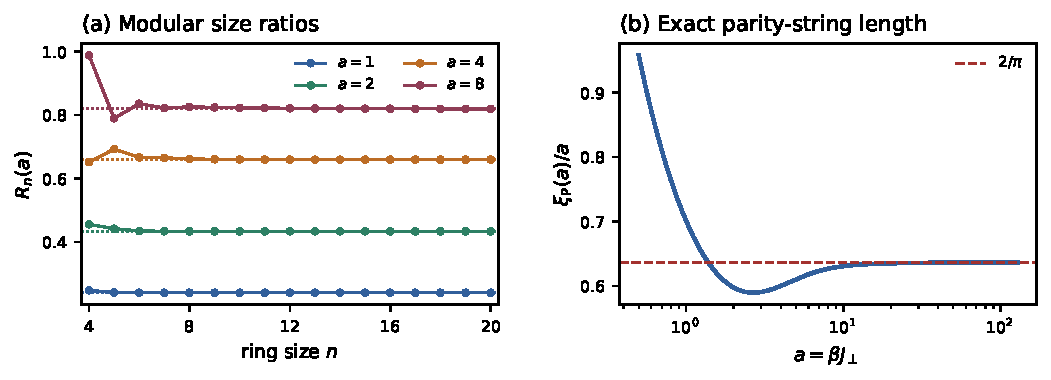
\includegraphics[width=\textwidth]{modular_flux_ring_attenuation.pdf}
 \caption{Thermal attenuation with ring length for the homogeneous-hopping
 family
 in Eq.~\eqref{eq:attenuation-family}.  (a) Consecutive-size ratios
 $R_n(a)$ from the exact Jordan--Wigner reconstruction.  Horizontal lines
 are the unfitted values $r_{\rm P}(a)$ from
 Eq.~\eqref{eq:parity-scale}.  (b) Exact parity-string length
 $\xi_{\rm P}(a)/a$ obtained from the integral.  The dashed line is the
 low-temperature limit $2/\pi$.  The modular data are evaluated only through
 $n=20$ in the figure.  The longer-size checks are given in
 Table~\ref{tab:attenuation-check}.}
 \label{fig:ring-attenuation}
\end{figure*}

\section{Comparison with two spin-chirality diagnostics}
\label{sec:comparison}

We now restrict the comparison to the axial spin-$1/2$ triangle.  The modular
response is best interpreted by comparing it with two quantities on the same
thermal state.  The first is the scalar spin chirality
\cite{WenWilczekZee1989},
\begin{equation}
 \chi_{ABC}=\bm S_A\cdot(\bm S_B\times\bm S_C).
 \label{eq:scalar-chirality}
\end{equation}
The second is the oriented loop of bond coherences
\begin{equation}
 G_\beta=\operatorname{Im}\left[
 \langle S_A^+S_B^-\rangle_\beta
 \langle S_B^+S_C^-\rangle_\beta
 \langle S_C^+S_A^-\rangle_\beta\right].
 \label{eq:coherence-loop}
\end{equation}
Unlike \eqref{eq:def-M}, $G_\beta$ presupposes the three bond operators and
the cycle whose flux is to be tested.

Direct expansion of the Gibbs state gives, on every oriented edge,
\begin{equation}
 \langle S_x^+S_y^-\rangle_\beta
 =-\frac{\beta}{8}\overline{t_{xy}}+O(\beta^2),
 \label{eq:coherence-leading}
\end{equation}
and hence
\begin{equation}
 G_\beta=\frac{\beta^3}{512}\PhiTri+O(\beta^4).
 \label{eq:G-leading}
\end{equation}
The leading term is gauge invariant, independent of all fields and all
longitudinal exchanges, and vanishes when the cycle is opened into a tree.

By contrast,
\begin{equation}
 \langle\chi_{ABC}\rangle_\beta
 =-\frac{\beta^2}{32}\left(
 h_AD_{BC}^z+h_BD_{CA}^z+h_CD_{AB}^z\right)+O(\beta^3).
 \label{eq:chi-leading}
\end{equation}
This is a sum of single-bond DM amplitudes.  The fixed laboratory operator
\eqref{eq:scalar-chirality} is not invariant under independent axial rotations
of the three local frames, and its leading thermal expectation can remain
nonzero on the open chain $A-B-C$, where the bond phases are removable
and \eqref{eq:def-M} vanishes exactly.

The comparison is summarized in Table~\ref{tab:diagnostics}.  On the narrow
task of measuring the flux of a chosen triangle, $G_\beta$ has a lower-order
onset in $\beta$ and does not require a magnetic field.  Among the three diagnostics
compared here, only the modular commutator is specified by the density matrix
and the tripartition alone.  More generally, its local-unitary invariance and
conjugation oddness imply that a nonzero value witnesses state chirality in
the sense of Ref.~\cite{VardhanEtAl2026}.  It does so without choosing a
microscopic loop operator.  The witness is not faithful.  A zero modular
commutator need not imply a local real structure or the absence of broader
many-body chirality \cite{EllisonEtAl2026}.

\begin{table}[b]
\caption{Leading high-temperature behavior on the axial spin-$1/2$ triangle.}
\label{tab:diagnostics}
\begin{ruledtabular}
\begin{tabular}{lccc}
Diagnostic & Order & Gauge invariant & Leading dependence\\
\hline
$\langle\chi_{ABC}\rangle_\beta$ & $\beta^2$ & no
& $\sum_x h_xD^z_{e\not\ni x}$\\
$G_\beta$ & $\beta^3$ & yes & $\PhiTri$\\
$\Mmod_\beta(AB,BC)$ & $\beta^4$ & yes & $h_B\PhiTri$\\
\end{tabular}
\end{ruledtabular}
\end{table}

\section{Finite-temperature crossover}
\label{sec:finite-temperature}

To connect the perturbative coefficients with the full thermal response, we
diagonalize two XY Hamiltonians.  The first is the minimal
triangle
\begin{equation}
 t_{AB}=t_{BC}=1,\qquad t_{CA}=\ii,\qquad
 h_A=h_C=0,\qquad h_B=0.7,
 \label{eq:numerical-triangle}
\end{equation}
and the second is the four-site ring
\begin{equation}
 (t_{AB},t_{BC},t_{CD},t_{DA})=(1,1,1,\ii),\qquad
 (h_A,h_B,h_C,h_D)=(0,0.7,0,0).
 \label{eq:numerical-square}
\end{equation}
All $J_e^z$ vanish, and energies are measured in units of $|t_{AB}|$.  The
reduced density matrices are formed from the exact Gibbs states and their
logarithms are evaluated spectrally.

Figure~\ref{fig:thermal-crossover}(a) displays both full responses.  The
triangle signal grows in magnitude from its quartic law, reaches a broad
minimum near $\beta=5.81$, and then returns to zero.  Panels (b) and (c) test
the triangle and square high-temperature coefficients without fitting.  For
the triangle,
\begin{align}
 m_4&=-\frac{0.7}{32},\nonumber\\
 m_6&=\frac{4(0.7)^3+8(0.7)+6(0.7)}{1536},
 \label{eq:numerical-m4m6}
\end{align}
while the square coefficient is
\begin{equation}
 m_5^\square=\frac{0.7}{128}.
 \label{eq:numerical-square-m5}
\end{equation}
The sextic triangle approximation tracks the exact ratio over a visibly
larger interval than the quartic constant alone.  At the point
\eqref{eq:numerical-triangle}, the XY quintic term vanishes and
$\operatorname{Im}(W_\triangle^2)=0$ also removes the septic term.  Thus the
residual after $m_4+\beta^2m_6$ starts at order $\beta^4$ in the plotted
ratio, providing a simultaneous numerical check of both cancellations.  For
the even four-site ring, the parity relation
$\Mmod_{-\beta}=-\Mmod_\beta$ implies
$\Mmod_\beta/\beta^5=m_5^\square+O(\beta^2)$, as observed in panel (c).

The opposite low-temperature limits have a state-theoretic explanation.  If
$ABC$ is the whole system and $\rho=|\psi\rangle\langle\psi|$ is pure, then
\begin{equation}
 \Mmod_\rho(AB,BC)=0,
 \label{eq:pure-state-zero}
\end{equation}
where the logarithms are restricted to the supports of the reduced states
\cite{ZouEtAl2022}.\footnote{Schmidt decomposition reduces the expectation to
$\langle\psi|[\log\rho_C,\log\rho_A]|\psi\rangle=0$.}
Consequently, for the triangle with a nondegenerate
ground state, $\Mmod_\beta\to0$ as $\beta\to\infty$.  Although the matrix
logarithm is singular at the rank-deficient boundary, the divergent reduced
eigenvalue logarithms grow at most linearly in $\beta$, whereas excited-state
weights are exponentially small in the finite spectral gap.

For the four-site ring, the union $AB\cup BC=ABC$ leaves the site $D$ outside
the measured regions.  The global ground state is pure and nondegenerate, but
its reduced state on $ABC$ is mixed, so Eq.~\eqref{eq:pure-state-zero} does not
apply.  At the point \eqref{eq:numerical-square}, the gap is
$0.2344774934$ and
\begin{equation}
 \lim_{\beta\to\infty}\Mmod_\beta(AB,BC)
 \simeq0.3146212191.
 \label{eq:square-ground-limit}
\end{equation}
This value is obtained by direct numerical evaluation of the nondegenerate
ground state.
The exterior spin leaves a mixed three-site ground-state reduction, allowing
a nonzero zero-temperature limit while the high-temperature loop hierarchy is
preserved.

\begin{figure*}[t]
 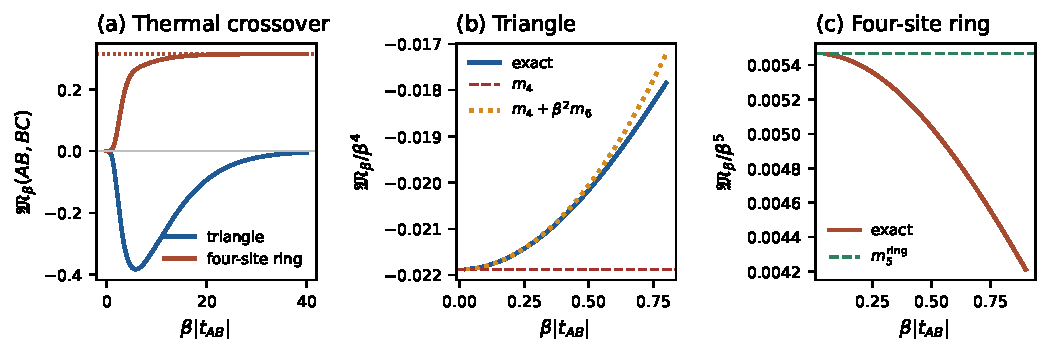
\includegraphics[width=\textwidth]{modular_flux_thermal_networks.pdf}
 \caption{Finite-temperature modular response for
 Eqs.~\eqref{eq:numerical-triangle} and \eqref{eq:numerical-square}.
 (a) Exact-diagonalization curves for the triangle and four-site ring.
 (b) Triangle ratio $\Mmod_\beta/\beta^4$ compared with $m_4$ and
 $m_4+\beta^2m_6$.  The residual is $O(\beta^4)$ because $m_5=m_7=0$ at
 this point.  (c) Four-site ratio $\Mmod_\beta/\beta^5$ compared with the
 exact coefficient $m_5^\square$.  The leading correction is $O(\beta^2)$.
 No fitted coefficient is used.}
 \label{fig:thermal-crossover}
\end{figure*}

\section{Measurement and scope}
\label{sec:discussion}

The results above deliberately assign a non-topological role to the modular
commutator.  Recent counterexamples show that it is not a universal extractor
of chiral central charge on arbitrary lattices \cite{GassLevin2024}, while
mixed-state topological phases require diagnostics beyond naive extensions of
pure-state probes \cite{SunEtAl2026}.  Our thermal statements make no such
claims.  They give finite-dimensional identities in specified spin models.
Within the axial class, the modular commutator is an exactly controlled joint
probe of a nonreal Wilson product and time-reversal breaking.  It is also a
nonfaithful witness of state chirality in the local-unitary sense of
Ref.~\cite{VardhanEtAl2026}.  This is compatible with the distinct
finite-depth notion of Ref.~\cite{EllisonEtAl2026}, which can remain nontrivial
when tripartite modular commutators vanish.

For three qubits, the quantity can in principle be reconstructed from state
tomography.  One estimates $\rho_{ABC}$, obtains $\rho_{AB}$ and $\rho_{BC}$
by partial trace, forms their matrix logarithms, and evaluates
Eq.~\eqref{eq:def-M}.  This state-intrinsic character
is also the source of its principal practical cost relative to $G_\beta$.
Matrix logarithms of estimated reduced states become poorly conditioned when small eigenvalues
approach zero.  More precisely, the Fr\'echet derivative obeys the scale
\begin{equation}
 \|D\log_\rho[\delta\rho]\|
 \le \frac{\|\delta\rho\|}{\lambda_{\min}(\rho)},
 \label{eq:log-conditioning}
\end{equation}
so low-temperature reconstruction requires precision that grows as
$\lambda_{\min}(\rho)$ decreases.  Protocols for entanglement-Hamiltonian
tomography have been demonstrated in quantum
simulators \cite{KokailEtAl2021}, while scalar chirality admits dedicated
measurement circuits \cite{ReascosEtAl2023}.  Axial DM spin models can also
be engineered in programmable platforms.  A Rydberg-atom construction using
Raman transitions and a rotating spin frame was proposed in
Ref.~\cite{KunimiEtAl2024}.  A full statistical error analysis for
Eq.~\eqref{eq:def-M} lies beyond the present work.

Theorem~\ref{thm:unicyclic-onset} assumes a finite, simple, connected,
unicyclic graph and the axial Hamiltonian \eqref{eq:axial-H}.  The spins,
longitudinal exchanges, longitudinal fields, and grafted trees are arbitrary.
The parameters are fixed as $\beta\to0$.  If its displayed prefactor
vanishes, the theorem identifies a zero leading admissible coefficient and
does not locate the first nonzero term.  Proposition~\ref{prop:primitive-cycle}
is a coefficient extraction at one primitive multidegree.  It is not an
all-orders decomposition by cycles.  Corollary~\ref{cor:girth-onset} concerns
only the first admissible order, even when shortest cycles overlap.  The exact
higher-order counterexamples in Sec.~\ref{sec:primitive-cycles} preclude a
general cactus law or unrestricted cycle additivity.

The axial assumption is substantive.  Section~\ref{sec:axial-boundary}
exhibits an open-link gauge invariant generated by transverse on-site fields.
It can occur before the primitive winding term.  The arbitrary-spin
unicyclic coefficient itself is unchanged when extracted as the coefficient
of $h_BW_\gamma$, since that extraction sets the transverse-field variables to
zero.  It need not dominate the complete response once those fields are
present.  We do not give a complete transverse-field classification or an
arbitrary-spin formula for the local background.

The XY ring has a direct locality interpretation.  Its fixed three-site
reduced state acquires the primitive cycle phase through a process that winds
around the complementary arc.  At high temperature the cost of each added
bond is explicit in Eq.~\eqref{eq:ring-product-form}.  At arbitrary
temperature, Lemma~\ref{lem:parity-determinant} identifies the exact scale of
the fermion-parity string.  The modular size ratios approach that scale over
the computed sizes.  We do not prove $R_n\to r_{\rm P}$.  We also do not extend
the arbitrary-temperature attenuation analysis to XXZ rings.

\section{Conclusion}
\label{sec:conclusion}

For every finite unicyclic axial network considered here, the first admissible
cycle coefficient is fixed by the cycle length, the field at the overlap, the
product of local spin moments, and the imaginary part of the Wilson product.
The result permits arbitrary irreducible spins, longitudinal exchanges,
longitudinal fields, grafted trees, and nonconsecutive marked sites.  The same
coefficient extraction isolates primitive sectors on general graphs and the
sum over shortest marked cycles at the first admissible order.  Exact
higher-order counterexamples show why these statements do not extend to an
all-orders cycle decomposition.

The local-real-structure and antiunitary vanishing principles are state-level
statements.  Corollaries~\ref{cor:real-gauge} and \ref{cor:zero-field}
translate them into the graph and parameter language of the axial
Hamiltonian class.  The winding theorem also requires that class.  Transverse
on-site fields generate a local open-link gauge invariant at order seven.  In
the seven-cycle example it
appears before the primitive cycle term.  A nonzero modular commutator outside
the axial class therefore need not identify a closed-loop phase.  The axial
hypothesis is consequently a substantive boundary of the onset theorem.

For the qubit XY ring, Jordan--Wigner fermionization reduces the full
finite-temperature calculation to one-particle matrices and fixed local
blocks.  The parity determinant and the asymptotics of $\xi_{\rm P}$ are
analytic.  The approach of the modular size ratios to $r_{\rm P}$ over the
computed sizes is numerical.  No large-size limit is claimed.  The XY-ring
calculation gives a finite-temperature instance relevant to the free-fermion
direction in Open Problem 3 of Ref.~\cite{KimEtAl2022PRB}.  The finite spin
networks give instances relevant to the few-body question in Open Problem 7.

Scalar chirality, a coherence Wilson loop, and the modular commutator probe
different information in the same axial qubit triangle.  The modular quantity
is less direct as a flux meter than the coherence loop.  It is also the only
one defined by the state and the tripartition alone.  Under the hypotheses
proved here,
this state-intrinsic quantity has an exact local, thermal, and geometric
interpretation whose limitations are explicit.

\section*{Data Availability}

The source code and exact-arithmetic certificates supporting this study will
be available in the accompanying GitHub repository at
\texttt{[GITHUB URL]}.  The repository version used for this article will be
archived on Zenodo under the version-specific DOI
\texttt{[ZENODO VERSION DOI]}.  The Zenodo concept DOI
\texttt{[ZENODO CONCEPT DOI]} will resolve the complete version history.  The
archive includes \path{SHA256SUMS_v06.txt}, which records SHA-256 checksums
for the deposited files.  No additional data were generated.

\appendix

\section{Exact Pauli certificate for the triangle}
\label{app:pauli-certificate}

At the parameter point \eqref{eq:arbitrary-triangle-point}, introduce
\begin{align}
 a&=H_{AB}=S_A^xS_B^x+S_A^yS_B^y,
 \label{eq:a-def}\\
 b&=H_{BC}=S_B^xS_C^x+S_B^yS_C^y,
 \label{eq:b-def}\\
 c&=H_{CA}=S_A^yS_C^x-S_A^xS_C^y,
 \label{eq:c-def}\\
 H_0&=a+b+c.
 \label{eq:H0-def}
\end{align}
The normalized trace is $\tau=\Tr/8$.  At zero field,
\begin{align}
 P_0&=a,
 &Q_0&=b,
 \label{eq:P0Q0}\\
 A_2^{(0)}
 &=\frac18I+\frac14(S_A^yS_B^x-S_A^xS_B^y),
 \label{eq:A20}\\
 B_2^{(0)}
 &=\frac18I+\frac14(S_B^yS_C^x-S_B^xS_C^y).
 \label{eq:B20}
\end{align}

Put
\begin{equation}
 H(h)=H_0+hH_1^{(r)},
 \qquad
 H_1^{(r)}=-S_r^z,
 \qquad r\in\{A,B,C\}.
 \label{eq:field-perturbation}
\end{equation}
The first derivatives of $P=\E_{AB}H$ and $Q=\E_{BC}H$ are
\begin{equation}
\begin{array}{c|cc}
 r&P_1^{(r)}&Q_1^{(r)}\\
 \hline
 A&-S_A^z&0\\
 B&-S_B^z&-S_B^z\\
 C&0&-S_C^z
\end{array}
\label{eq:P1Q1-table}
\end{equation}
Since $\{S^z,S^x\}=\{S^z,S^y\}=0$ for spin $1/2$, direct substitution into
Eqs.~\eqref{eq:A2} and \eqref{eq:B2} gives
\begin{equation}
 \left.\frac{dA_2}{dh}\right|_{h=0}
 =\left.\frac{dB_2}{dh}\right|_{h=0}=0
 \label{eq:A2B2-derivatives}
\end{equation}
for all three choices of $r$.

Write the three terms on the right-hand side of
Eq.~\eqref{eq:m4-general} as
\begin{align}
 T_0&=\frac{\ii}{2}\tau(H^2[P,Q]),
 \label{eq:T0}\\
 T_1&=\ii\tau(H[P,B_2]),
 \label{eq:T1}\\
 T_2&=\ii\tau(H[A_2,Q]).
 \label{eq:T2}
\end{align}
Their field derivatives at zero are
\begin{align}
 \left.\frac{dT_0}{dh}\right|_0
 &=\frac{\ii}{2}\tau\left(
 \{H_0,H_1^{(r)}\}[P_0,Q_0]
 +H_0^2\bigl([P_1^{(r)},Q_0]+[P_0,Q_1^{(r)}]\bigr)
 \right),
 \label{eq:T0-derivative}\\
 \left.\frac{dT_1}{dh}\right|_0
 &=\ii\tau\left(
 H_1^{(r)}[P_0,B_2^{(0)}]
 +H_0[P_1^{(r)},B_2^{(0)}]
 \right),
 \label{eq:T1-derivative}\\
 \left.\frac{dT_2}{dh}\right|_0
 &=\ii\tau\left(
 H_1^{(r)}[A_2^{(0)},Q_0]
 +H_0[A_2^{(0)},Q_1^{(r)}]
 \right).
 \label{eq:T2-derivative}
\end{align}

For $r=B$, the required Pauli identities are
\begin{align}
 [a,b]
 &=\ii S_B^z(S_A^xS_C^y-S_A^yS_C^x)
 =-\ii S_B^zc,
 \label{eq:ab-commutator}\\
 \{a,c\}
 &=\frac12(S_B^yS_C^x-S_B^xS_C^y),
 \label{eq:ac-anticommutator}\\
 \{b,c\}
 &=\frac12(S_A^yS_B^x-S_A^xS_B^y).
 \label{eq:bc-anticommutator}
\end{align}
Moreover,
\begin{equation}
 C_1^{(B)}
 =[-S_B^z,b]+[a,-S_B^z]
 =\ii\left(
 S_B^xS_C^y-S_B^yS_C^x
 +S_A^xS_B^y-S_A^yS_B^x
 \right).
 \label{eq:C1B}
\end{equation}
Because $\{a,S_B^z\}=\{b,S_B^z\}=0$ and
$\{c,S_B^z\}=2cS_B^z$, the first part of
Eq.~\eqref{eq:T0-derivative} is
\begin{equation}
 \frac{\ii}{2}\tau\left(-\{H_0,S_B^z\}[a,b]\right)
 =-\tau\bigl(c^2(S_B^z)^2\bigr)
 =-\frac1{32}.
 \label{eq:T0B-first}
\end{equation}
Only the anticommutators \eqref{eq:ac-anticommutator} and
\eqref{eq:bc-anticommutator} contribute to
$\tau(H_0^2C_1^{(B)})$.  Each orientation gives $1/32$ after multiplication
by $\ii/2$, hence
\begin{equation}
 \frac{\ii}{2}\tau(H_0^2C_1^{(B)})=\frac1{16}.
 \label{eq:T0B-second}
\end{equation}
Combining Eqs.~\eqref{eq:T0B-first} and \eqref{eq:T0B-second} yields
\begin{equation}
 \left.\frac{dT_0}{dh}\right|_{0,r=B}=\frac1{32}.
 \label{eq:T0B-total}
\end{equation}

Equations \eqref{eq:A20} and \eqref{eq:B20} also give
\begin{equation}
 [-S_B^z,B_2^{(0)}]=\frac{\ii}{4}b,
 \qquad
 [A_2^{(0)},-S_B^z]=\frac{\ii}{4}a.
 \label{eq:A2B2-B-commutators}
\end{equation}
The remaining terms in Eqs.~\eqref{eq:T1-derivative} and
\eqref{eq:T2-derivative} vanish by local Pauli orthogonality.  Since
$\tau(a^2)=\tau(b^2)=1/8$, one finds
\begin{equation}
 \left.\frac{dT_1}{dh}\right|_{0,r=B}
 =\left.\frac{dT_2}{dh}\right|_{0,r=B}
 =-\frac1{32}.
 \label{eq:T1T2B}
\end{equation}

For $r=A$, one has $Q_1^{(A)}=0$ and
$[P_1^{(A)},Q_0]=0$.  Furthermore,
\(
\{H_0,S_A^z\}=2bS_A^z
\),
and every remaining trace contains on $A$ either $S_A^zS_A^x$ or
$S_A^zS_A^y$.  It therefore vanishes.  The $r=C$ calculation is the reflected
counterpart.  Altogether,
\begin{equation}
\begin{array}{c|ccc|c}
 r&dT_0/dh&dT_1/dh&dT_2/dh&dm_4/dh\\
 \hline
 A&0&0&0&0\\
 B&1/32&-1/32&-1/32&-1/32\\
 C&0&0&0&0
\end{array}
\label{eq:certificate-table}
\end{equation}
This is the spin-$1/2$ specialization of
Eq.~\eqref{eq:arbitrary-spin-contraction-table}.

\section{Exact identification of the fifth- through seventh-order coefficients}
\label{app:higher-orders}

The higher coefficients were obtained without floating-point arithmetic.  For
a truncation order $N$, we form
\begin{equation}
 r_\beta=
 \frac{\displaystyle\sum_{n=0}^N\frac{(-\beta)^n}{n!}H^n}
 {\displaystyle\tau\left(\sum_{n=0}^N\frac{(-\beta)^n}{n!}H^n\right)}
 +O(\beta^{N+1})
 \label{eq:exact-r-series}
\end{equation}
and use the finite series
\begin{equation}
 L_X(\beta)=
 \sum_{p=1}^N\frac{(-1)^{p+1}}{p}
 \left(\E_X(r_\beta)-I\right)^p+O(\beta^{N+1}).
 \label{eq:exact-log-series}
\end{equation}
Substitution into Eq.~\eqref{eq:M-normalized} reduces every coefficient to
Pauli matrix products with entries in $\mathbb Q(\ii)$.

For $m_5$, the classification \eqref{eq:m5-classification} leaves nine
constants.  Setting $t=(1,1,\ii)$ and turning on one $J_e^z$ at a time gives,
in units of $1/384$,
\begin{equation}
\begin{array}{c|rrr}
 &J_{AB}^z&J_{BC}^z&J_{CA}^z\\
\hline
h_A&3&-2&0\\
h_B&-1&-1&-3\\
h_C&-2&3&0
\end{array}
\label{eq:m5-coefficient-table}
\end{equation}
which is Eq.~\eqref{eq:m5-exact}.  Reflection
$A\leftrightarrow C$ together with $AB\leftrightarrow BC$ provides an
independent covariance check.

For the XY sextic sector, write
\begin{equation}
 \frac{m_6}{\PhiTri}=p_3(h_A,h_B,h_C)
 +\sum_{x,e}b_{x,e}h_x|t_e|^2,
 \label{eq:m6-ansatz}
\end{equation}
where $p_3$ is cubic.  The cubic part is already determined at one nonzero
flux point and is found to be
\begin{equation}
 p_3=\frac{h_B(h_A^2+h_Ah_C+h_B^2+h_C^2)}{384}.
 \label{eq:m6-cubic}
\end{equation}
The nine linear-amplitude coefficients are fixed from the three configurations
whose squared amplitudes form
\begin{equation}
 \mathcal C=
 \begin{pmatrix}
 1&1&1\\
 4&1&1\\
 1&1&4
 \end{pmatrix},
 \qquad \det\mathcal C=-9.
 \label{eq:calibration-matrix}
\end{equation}
The exact solution is
\begin{equation}
\begin{array}{c|ccc}
 &|t_{AB}|^2&|t_{BC}|^2&|t_{CA}|^2\\
\hline
h_A&1/1536&0&0\\
h_B&1/384&1/384&1/256\\
h_C&0&1/1536&0
\end{array}.
\label{eq:m6-coefficient-table}
\end{equation}
Equations~\eqref{eq:m6-cubic} and \eqref{eq:m6-coefficient-table} reproduce
the hopping polynomial \eqref{eq:Pperp}.  Four additional hopping
configurations, not used in the identification, were checked against the
closed form.

The remaining sextic sector is quadratic in longitudinal exchanges.  In
units of $\PhiTri/1536$, its eighteen coefficients are
\begin{equation}
\begin{array}{c|rrr|rrr}
 &(J_{AB}^z)^2&(J_{BC}^z)^2&(J_{CA}^z)^2
 &J_{AB}^zJ_{BC}^z&J_{BC}^zJ_{CA}^z&J_{AB}^zJ_{CA}^z\\
\hline
h_A&1&0&0&0&-4&3\\
h_B&1&1&2&1&-1&-1\\
h_C&0&1&0&0&3&-4
\end{array}
\label{eq:m6-Jz-table}
\end{equation}
Six configurations of $(J_{AB}^z,J_{BC}^z,J_{CA}^z)$ isolate these six
quadratic monomials while retaining symbolic fields.  Two additional generic
choices with $t_e\in\mathbb Q(\ii)$ and $J_e^z\in\mathbb Q$, not used in the
calibration, reproduce Eq.~\eqref{eq:Pz} exactly.  This establishes the full
sextic formula \eqref{eq:m6-exact}.

Finally, in the XY model the degree-seven classification leaves
three constants:
\begin{equation}
 m_7=\operatorname{Im}(W_\triangle^2)
 (q_Ah_A+q_Bh_B+q_Ch_C).
 \label{eq:m7-ansatz}
\end{equation}
Exact evaluation with symbolic fields and $t_e\in\mathbb Q(\ii)$ at a point with
$\operatorname{Im}(W_\triangle^2)=1440$ gives
\begin{equation}
 (q_A,q_B,q_C)=-\frac1{92160}(2,41,2).
 \label{eq:m7-coefficients}
\end{equation}
A second generic point with
$\operatorname{Im}(W_\triangle^2)=-378$ and the unit-amplitude parameter
point $(1,1,\ii)$, where this invariant vanishes, provide two exact checks.

\section{Exact four-site coefficient certificate}
\label{app:ring-certificate}

The formal construction from \eqref{eq:exact-r-series} through
\eqref{eq:exact-log-series} also applies to the $16\times16$ four-site
Hamiltonian.  With symbolic $h_A,h_B,h_C,h_D$ and exact arithmetic over
$\mathbb Q(\ii)$, evaluation at the XY point $(1,1,1,\ii)$ gives
\begin{equation}
 [\beta^5]\Mmod_\beta(AB,BC)=\frac{h_B}{128},
 \qquad
 [h_A]=[h_C]=[h_D]=0.
 \label{eq:square-certificate}
\end{equation}
Replacing $t_{AB}=1$ by $t_{AB}=2$ doubles the result.  Gauge-flow grading at
degree five permits only
$\operatorname{Im}W_4\sum_xc_xh_x$.  Hence these evaluations determine all
four constants and reproduce Corollary~\ref{thm:square}.  Generic rational
longitudinal exchanges provide an additional exact check: they cannot enter
the degree-five winding monomial because its four hopping factors and one
field already exhaust the degree.

\section{Exact fermionic reconstruction of XY rings}
\label{app:fermionic-ring}

We give the details behind Proposition~\ref{prop:JW-reconstruction}.  Let
$c_j$ be Jordan--Wigner fermions ordered from $0$ to $n-1$, let
$\widehat p=(-1)^{N_f}$, and write
\begin{equation}
 S_j^z=c_j^\dagger c_j-\frac12,
 \qquad
 S_{n-1}^+S_0^-=-\widehat p\,c_{n-1}^\dagger c_0.
 \label{eq:JW-boundary}
\end{equation}
All bulk strings cancel.  In the sector $\widehat p=p$, the Hamiltonian is
$Q_p+\kappa_h$, where $Q_p=c^\dagger E_pc$,
$\kappa_h=\frac12\sum_jh_j$, and $E_p$ is the one-particle matrix specified below
Eq.~\eqref{eq:Gaussian-pieces}.  The projectors
$\Pi_p=(I+p\widehat p)/2$ give
\begin{align}
 e^{-\beta H_n}
 &=\frac{e^{-\beta\kappa_h}}2\sum_{p=\pm1}
 \left(e^{-\beta Q_p}+p\widehat p\,e^{-\beta Q_p}\right),
 \label{eq:parity-projectors}\\
 \widehat p\,e^{-\beta Q_p}
 &=e^{-c^\dagger(\beta E_p-\ii\pi I)c}.
 \label{eq:parity-insertion}
\end{align}
Thus the four matrices in Eq.~\eqref{eq:Gaussian-pieces} arise directly from
the two parity sectors, with and without a parity insertion.  The scalar
$e^{-\beta\kappa_h}/2$ cancels on normalization.

For any matrix $M$, the number-conserving Gaussian operator satisfies
\begin{equation}
 T(M):=\Tr G(M)=\det(I+e^{-M}),
 \qquad C(M)=(e^M+I)^{-1}.
 \label{eq:Gaussian-trace}
\end{equation}
When $T(M)\ne0$, the normalized operator $G(M)/T(M)$ reduces on a contiguous
set $\mathcal B$ to the Gaussian operator whose correlation matrix is the
principal submatrix $C(M)|_{\mathcal B}$.  Equation~\eqref{eq:Gamma-block}
is preferable because it remains regular at zeros of a parity-inserted
trace.  Indeed, $G(M_{p,1})=\widehat p\,e^{-\beta Q_p}$ is regular even
though $T(M_{p,1})=\det(I-e^{-\beta E_p})$ vanishes at $\beta=0$.

We now derive the bulk scale used in
Eqs.~\eqref{eq:parity-scale} through \eqref{eq:parity-low-T}.  In a zero-field
homogeneous ring, the eigenvalues of $E_p$ are
$J_\perp\cos k_m$, where the parity and the total flux only shift the
uniform momentum grid.  Lemma~\ref{lem:parity-determinant} therefore gives
\begin{equation}
 \lim_{n\to\infty}\frac1n
 \log\left|\frac{T_{p,1}}{T_{p,0}}\right|
 =\frac1{2\pi}\int_{-\pi}^{\pi}
 \log\left|\tanh\!\left(\frac a2\cos k\right)\right|\,dk
 =\log r_{\rm P}(a).
 \label{eq:parity-bulk-limit}
\end{equation}
The logarithmic singularities at the two Fermi points are integrable.  A
momentum grid that meets a zero is understood by a limiting twist.  Thus
$\xi_{\rm P}$ is the attenuation length of the thermal fermion-parity
insertion around the homogeneous ring.

For $a\to0$, the expansion
\begin{equation}
 \log|\tanh x|
 =\log|x|-\frac{x^2}{3}+\frac{7x^4}{90}+O(x^6)
 \label{eq:log-tanh-small}
\end{equation}
together with
$(2\pi)^{-1}\int_{-\pi}^{\pi}\log|\cos k|\,dk=-\log2$ yields
\begin{equation}
 \log r_{\rm P}(a)
 =\log\frac a4-\frac{a^2}{24}
 +\frac{7a^4}{3840}+O(a^6),
 \label{eq:parity-high-T-log}
\end{equation}
which implies Eq.~\eqref{eq:parity-high-T}.  For $a\to\infty$, only
neighborhoods of $k=\pm\pi/2$ contribute algebraically.  Rescaling their
local coordinate by $x=a(k\mp\pi/2)/2$ and using
\begin{equation}
 \int_{-\infty}^{\infty}-\log|\tanh x|\,dx=\frac{\pi^2}{4}
 \label{eq:tanh-integral}
\end{equation}
gives
\begin{equation}
 -\log r_{\rm P}(a)=\frac{\pi}{2a}+O(a^{-3}),
 \label{eq:parity-low-T-log}
\end{equation}
and hence Eq.~\eqref{eq:parity-low-T}.

Table~\ref{tab:attenuation-check} records the numerical comparison between
the exact factor $r_{\rm P}(a)$ and the last consecutive-size ratio computed
from the full modular functional in the family
\eqref{eq:attenuation-family}.  The adaptive cutoff keeps the modular signal
above the double-precision roundoff floor.  Increasing the cutoff gives the
displayed finite-size approach until that floor is reached.

\begin{table}[t]
\caption{Large-size numerical check of the parity-string attenuation scale.
$R_N(a)$ is computed from the Jordan--Wigner reconstruction, whereas
$r_{\rm P}(a)$ is evaluated independently from
Eq.~\eqref{eq:parity-scale}.}
\label{tab:attenuation-check}
\begin{ruledtabular}
\begin{tabular}{cccc}
$a$ & $N$ & $R_N(a)$ & $r_{\rm P}(a)$\\
\hline
$0.5$ & $13$ & $0.123718566605$ & $0.123718566605$\\
$1$   & $18$ & $0.240210848508$ & $0.240210848508$\\
$2$   & $25$ & $0.433416769933$ & $0.433416769933$\\
$4$   & $35$ & $0.659386662495$ & $0.659386662495$\\
$8$   & $50$ & $0.819227344995$ & $0.819227344443$\\
$16$  & $70$ & $0.906193444199$ & $0.906193409422$\\
\end{tabular}
\end{ruledtabular}
\end{table}

For the displayed cutoffs, the relative discrepancy is below
$4\times10^{-8}$ throughout and below $10^{-12}$ for $a\le4$.  The larger
residuals at $a=8$ and $16$ reflect the slower finite-size stabilization.

With $F_m$ as defined before Proposition~\ref{prop:JW-reconstruction},
taking a partial trace of Eq.~\eqref{eq:parity-projectors} proves
Eq.~\eqref{eq:rho-block-JW}.  In particular, with
$D$ from Eq.~\eqref{eq:Gamma-block},
\begin{align}
 \rho_{ABC}&=F_3\frac{\sum_{p,s}p^s\Gamma_{ABC}(M_{p,s})}{D}F_3,
 \label{eq:rhoABC-JW}\\
 \rho_{AB}&=\Tr_C\rho_{ABC},
 &\rho_{BC}&=\Tr_A\rho_{ABC}.
 \label{eq:rhoABBC-JW}
\end{align}
The desired quantity is then the fixed-size expression
\begin{equation}
 \Mmod_\beta(AB,BC)=\ii\Tr\rho_{ABC}
 \left[\log\rho_{AB}\otimes I_C,
 I_A\otimes\log\rho_{BC}\right].
 \label{eq:M-JW-closed}
\end{equation}
The only matrices whose dimension grows with $n$ are $E_p$ and their matrix
functions.  Hence the $O(n^3)$ cost quoted in Proposition~\ref{prop:JW-reconstruction}.

We finally record the parity relation used in Corollary~\ref{thm:ring-law}.
Complex conjugation in the spin basis gives
\begin{equation}
 \Mmod_\beta(\overline t,h)=-\Mmod_\beta(t,h).
 \label{eq:ring-conjugation}
\end{equation}
For even $n$, the on-site unitary
\begin{equation}
 U=(\sigma^x)^{\otimes n}\prod_{j=0}^{n-1}e^{\ii\pi jS_j^z}
 \label{eq:even-ring-U}
\end{equation}
obeys $UH_n(t,h)U^\dagger=-H_n(\overline t,h)$.  Local-unitary invariance and
Eq.~\eqref{eq:ring-conjugation} therefore imply
\begin{equation}
 \Mmod_{-\beta}(t,h)=-\Mmod_\beta(t,h),
 \qquad n\ \text{even}.
 \label{eq:even-ring-parity}
\end{equation}
For odd $n$ and $\operatorname{Re}W_n=0$, phases $\alpha_j$ can instead be
chosen so that
$e^{\ii(\alpha_j-\alpha_{j+1})}=-\overline t_j/t_j$ around the cycle.  The
product unitary $\prod_je^{-\ii\alpha_jS_j^z}\sigma_j^x$ then maps $H_n$ to
$-H_n$, giving
\begin{equation}
 \Mmod_{-\beta}(t,h)=\Mmod_\beta(t,h),
 \qquad n\ \text{odd},\quad\operatorname{Re}W_n=0.
 \label{eq:odd-ring-parity}
\end{equation}
These identities justify the parity-restricted high-precision extraction
used as an independent check.  At
$t=(1,\ldots,1,\ii)$ and $h_B=1$, calculations with 80-digit arithmetic for
$3\le n\le12$ reproduce
$2^{2n-1}[\beta^{n+1}]\Mmod_\beta=(-1)^n$ with maximum relative discrepancy
$1.3\times10^{-19}$.  Exact diagonalization and the fermionic reconstruction
agree at machine precision for $3\le n\le7$ with generic complex couplings
and fields.

\section{Computational validation}
\label{app:reproducibility}

The analytic proofs of Theorem~\ref{thm:unicyclic-onset},
Proposition~\ref{prop:primitive-cycle}, and Corollary~\ref{cor:girth-onset} do
not rely on computational interpolation.  The finite-dimensional coefficient
identities in Propositions~\ref{prop:local-transverse-sector} and
\ref{prop:complete-local-m7} are obtained by exhaustive exact-arithmetic
expansions of the normalized Gibbs state and reduced logarithms.  Further
exact certificates test the arbitrary-spin factor, nonconsecutive marked
sites, tree pruning, primitive-cycle coefficients, and the stated
higher-order obstructions.  One implementation uses exact SymPy arithmetic
\cite{MeurerEtAl2017}.  A separately written standard-library implementation
reproduces the formal-series calculations.  It is an independent
implementation of the same method, not an independent mathematical method.

Direct Gibbs-series evaluations, exact diagonalization, and the four-component
fermionic reconstruction provide numerical cross-checks.  High-precision
calculations independently check the leading ring coefficient and the
parity-restricted series.  The analytic attenuation formula, both of its
stated asymptotic regimes, every tabulated value, and all plotted data are
also checked before output is written.  No fitted coefficient is used.  The
repository and the versioned archive identified in the Data Availability
Statement contain the complete source code, exact test points, expected
outputs, dependency and execution information, and a SHA-256 manifest of the
deposited file set.

\begin{thebibliography}{99}

\bibitem{KimEtAl2022PRL}
I.~H.~Kim, B.~Shi, K.~Kato, and V.~V.~Albert,
``Chiral central charge from a single bulk wave function,''
Phys. Rev. Lett. \textbf{128}, 176402 (2022).

\bibitem{KimEtAl2022PRB}
I.~H.~Kim, B.~Shi, K.~Kato, and V.~V.~Albert,
``Modular commutator in gapped quantum many-body systems,''
Phys. Rev. B \textbf{106}, 075147 (2022).

\bibitem{ZouEtAl2022}
Y.~Zou, B.~Shi, J.~Sorce, I.~T.~Lim, and I.~H.~Kim,
``Modular commutators in conformal field theory,''
Phys. Rev. Lett. \textbf{129}, 260402 (2022).

\bibitem{Fan2022}
R.~Fan,
``From entanglement generated dynamics to the gravitational anomaly and
chiral central charge,''
Phys. Rev. Lett. \textbf{129}, 260403 (2022).

\bibitem{ParkEtAl2025}
S.-M.~Park, I.~H.~Kim, and E.-G.~Moon,
``Geometric additivity of the modular commutator for multipartite
entanglement,''
Phys. Rev. B \textbf{111}, 075167 (2025).

\bibitem{GassLevin2026}
J.~Gass and M.~Levin,
``R\'enyi-like entanglement probe of the chiral central charge,''
Phys. Rev. B \textbf{113}, 235136 (2026).

\bibitem{Zang2026}
Y.~Zang,
``Entanglement measure response to modular flow and chiral topological
phases,''
Phys. Rev. B \textbf{114}, 115124 (2026).

\bibitem{Zeng2026}
M.~Zeng,
``Parity anomaly as modular commutator with massless Dirac fermion,''
arXiv:2608.26078 (2026).

\bibitem{ShefferEtAl2026}
Y.~Sheffer, R.~Fan, A.~Stern, E.~Berg, and S.~Ryu,
``Probing chiral topological states with permutation defects,''
Phys. Rev. B \textbf{113}, 195123 (2026).

\bibitem{MaityEtAl2025}
A.~Maity, A.~Kumar, and V.~Tripathi,
``Identifying chiral topological order in microscopic spin models by modular
commutator,''
arXiv:2510.06086 (2025).

\bibitem{GassLevin2024}
J.~Gass and M.~Levin,
``Many-body systems with spurious modular commutators,''
Phys. Rev. Lett. \textbf{133}, 256604 (2024).

\bibitem{SunEtAl2026}
S.~Sun, B.~Aldossari, R.~Devkota, and Z.-X.~Luo,
``Measures of chirality in mixed-state topological phases,''
arXiv:2606.26235 (2026).

\bibitem{VardhanEtAl2026}
S.~Vardhan, B.~Shi, I.~H.~Kim, and Y.~Zou,
``Chirality, magic, and quantum correlations in multipartite quantum
states,''
SciPost Phys. \textbf{20}, 066 (2026).

\bibitem{FernandesEtAl2024}
C.~Fernandes, R.~Wagner, L.~Novo, and E.~F.~Galv\~ao,
``Unitary-invariant witnesses of quantum imaginarity,''
Phys. Rev. Lett. \textbf{133}, 190201 (2024).

\bibitem{EllisonEtAl2026}
T.~D.~Ellison, D.~Lee, Z.~Li, A.~Moharramipour, Y.~Panahi, and B.~Yoshida,
``Many-body chirality of topological stabilizer states,''
arXiv:2606.20472 (2026).

\bibitem{Dzyaloshinsky1958}
I.~Dzyaloshinsky,
``A thermodynamic theory of `weak' ferromagnetism of antiferromagnetics,''
J. Phys. Chem. Solids \textbf{4}, 241--255 (1958).

\bibitem{Moriya1960}
T.~Moriya,
``Anisotropic superexchange interaction and weak ferromagnetism,''
Phys. Rev. \textbf{120}, 91--98 (1960).

\bibitem{JordanWigner1928}
P.~Jordan and E.~Wigner,
``\"Uber das Paulische \"Aquivalenzverbot,''
Z. Phys. \textbf{47}, 631--651 (1928).

\bibitem{LiebSchultzMattis1961}
E.~Lieb, T.~Schultz, and D.~Mattis,
``Two soluble models of an antiferromagnetic chain,''
Ann. Phys. (N.Y.) \textbf{16}, 407--466 (1961).

\bibitem{WenWilczekZee1989}
X.~G.~Wen, F.~Wilczek, and A.~Zee,
``Chiral spin states and superconductivity,''
Phys. Rev. B \textbf{39}, 11413--11423 (1989).

\bibitem{KokailEtAl2021}
C.~Kokail, R.~van Bijnen, A.~Elben, B.~Vermersch, and P.~Zoller,
``Entanglement Hamiltonian tomography in quantum simulation,''
Nat. Phys. \textbf{17}, 936--942 (2021).

\bibitem{ReascosEtAl2023}
L.~I.~Reascos, B.~Murta, E.~F.~Galv\~ao, and J.~Fern\'andez-Rossier,
``Quantum circuits to measure scalar spin chirality,''
Phys. Rev. Research \textbf{5}, 043087 (2023).

\bibitem{KunimiEtAl2024}
M.~Kunimi, T.~Tomita, H.~Katsura, and Y.~Kato,
``Proposal for simulating quantum spin models with the
Dzyaloshinskii--Moriya interaction using Rydberg atoms and the construction of
asymptotic quantum many-body scar states,''
Phys. Rev. A \textbf{110}, 043312 (2024).

\bibitem{MeurerEtAl2017}
A.~Meurer \textit{et al.},
``SymPy: Symbolic computing in Python,''
PeerJ Comput. Sci. \textbf{3}, e103 (2017).

\end{thebibliography}

\end{document}
